\documentclass[11pt]{book}
\usepackage[T1]{fontenc}
\usepackage[utf8]{inputenc}
\usepackage{lmodern}
\usepackage{hyperref}
\usepackage{graphicx}
\usepackage[english]{babel}
\usepackage{listings}
\usepackage{amsmath}
\usepackage{amsthm}
\usepackage{amssymb}
\usepackage{natbib}
\usepackage{stmaryrd}
\usepackage{xypic}
\usepackage{semantic}
\usepackage{wrapfig}

%% For pictures
\usepackage{tikz}
\usetikzlibrary{arrows.meta}
\tikzset{baseline=(current bounding box.center), >/.tip={Triangle[scale=1.4]}}

% Computer Modern is already the default. -Jeremy
%\renewcommand{\ttdefault}{cmtt}

\lstset{%
language=Lisp,
basicstyle=\ttfamily\small,
escapechar=|,
columns=flexible
}

\newtheorem{theorem}{Theorem}
\newtheorem{lemma}[theorem]{Lemma}
\newtheorem{corollary}[theorem]{Corollary}
\newtheorem{proposition}[theorem]{Proposition}
\newtheorem{constraint}[theorem]{Constraint}
\newtheorem{definition}[theorem]{Definition}
\newtheorem{exercise}[theorem]{Exercise}

%%%%%%%%%%%%%%%%%%%%%%%%%%%%%%%%%%%%%%%%%%%%%%%%%%%%%%%%%%%%%%%%%%%%%%%%%%%%%%%%
% 'dedication' environment: To add a dedication paragraph at the start of book %
% Source: http://www.tug.org/pipermail/texhax/2010-June/015184.html            %
%%%%%%%%%%%%%%%%%%%%%%%%%%%%%%%%%%%%%%%%%%%%%%%%%%%%%%%%%%%%%%%%%%%%%%%%%%%%%%%%
\newenvironment{dedication}
{
   \cleardoublepage
   \thispagestyle{empty}
   \vspace*{\stretch{1}}
   \hfill\begin{minipage}[t]{0.66\textwidth}
   \raggedright
}
{
   \end{minipage}
   \vspace*{\stretch{3}}
   \clearpage
}

%%%%%%%%%%%%%%%%%%%%%%%%%%%%%%%%%%%%%%%%%%%%%%%%
% Chapter quote at the start of chapter        %
% Source: http://tex.stackexchange.com/a/53380 %
%%%%%%%%%%%%%%%%%%%%%%%%%%%%%%%%%%%%%%%%%%%%%%%%
\makeatletter
\renewcommand{\@chapapp}{}% Not necessary...
\newenvironment{chapquote}[2][2em]
  {\setlength{\@tempdima}{#1}%
   \def\chapquote@author{#2}%
   \parshape 1 \@tempdima \dimexpr\textwidth-2\@tempdima\relax%
   \itshape}
  {\par\normalfont\hfill--\ \chapquote@author\hspace*{\@tempdima}\par\bigskip}
\makeatother

%%%%%%%%%%%%%%%%%%%%%%%%%%%%%%%%%%%%%%%%%%%%%%%%%%%%%%%%%%%%%%%%%%%%%%%%%%%%%%%%

\newcommand{\itm}[1]{\ensuremath{\mathit{#1}}}
\newcommand{\ttm}[1]{\ensuremath{\mathtt{#1}}}
\newcommand{\Stmt}{\itm{stmt}}
\newcommand{\Exp}{\itm{exp}}
\newcommand{\Def}{\itm{def}}
\newcommand{\Type}{\itm{type}}
\newcommand{\FType}{\itm{ftype}}
\newcommand{\Instr}{\itm{instr}}
\newcommand{\Block}{\itm{block}}
\newcommand{\Tail}{\itm{tail}}
\newcommand{\Prog}{\itm{prog}}
\newcommand{\Arg}{\itm{arg}}
\newcommand{\Atm}{\itm{atm}}
\newcommand{\Reg}{\itm{reg}}
\newcommand{\Int}{\itm{int}}
\newcommand{\Var}{\itm{var}}
\newcommand{\Op}{\itm{op}}
\newcommand{\key}[1]{\texttt{#1}}
\newcommand{\code}[1]{\texttt{#1}}

\newcommand{\LP}[0]{\key{(}}
\newcommand{\RP}[0]{\key{)}}
\newcommand{\LS}[0]{\key{[}}
\newcommand{\RS}[0]{\key{]}}
\newcommand{\INT}[1]{\key{(Int}\;#1\key{)}}
\newcommand{\BOOL}[1]{\key{(Bool}\;#1\key{)}}
\newcommand{\PRIM}[2]{\LP\key{Prim}~#1~\LP\key{list}~#2\RP\RP}
\newcommand{\READ}{\key{(Prim}\;\code{'read}\;\key{'())}}
\newcommand{\CREAD}{\key{(read)}}
\newcommand{\NEG}[1]{\key{(Prim}\;\code{'-}\;\code{(list}\;#1\;\code{))}}
\newcommand{\CNEG}[1]{\LP\key{-}~#1\RP}
\newcommand{\PROGRAM}[2]{\LP\code{Program}\;#1\;#2\RP}
\newcommand{\PROGRAMDEFSEXP}[3]{\code{(ProgramDefsExp}~#1~#2~#3\code{)}}
\newcommand{\PROGRAMDEFS}[2]{\code{(ProgramDefs}~#1~#2\code{)}}
\newcommand{\ADD}[2]{\key{(Prim}\;\code{'+}\;\code{(list}\;#1\;#2\code{))}}
\newcommand{\CADD}[2]{\LP\key{+}~#1~#2\RP}
\newcommand{\SUB}[2]{\key{(Prim}\;\code{'-}\;\code{(list}\;#1\;#2\code{))}}
\newcommand{\CSUB}[2]{\LP\key{-}~#1~#2\RP}
\newcommand{\CWHILE}[2]{\LP\key{while}~#1~#2\RP}
\newcommand{\WHILE}[2]{\LP\key{WhileLoop}~#1~#2\RP}
\newcommand{\CBEGIN}[2]{\LP\key{begin}~#1~#2\RP}
\newcommand{\BEGIN}[2]{\LP\key{Begin}~#1~#2\RP}
\newcommand{\CSETBANG}[2]{\LP\key{set!}~#1~#2\RP}
\newcommand{\SETBANG}[2]{\LP\key{SetBang}~#1~#2\RP}
\newcommand{\AND}[2]{\key{(Prim}\;\code{'and}\;\code{(list}\;#1\;#2\code{))}}
\newcommand{\OR}[2]{\key{(Prim}\;\code{'or}\;\code{(list}\;#1\;#2\code{))}}
\newcommand{\NOT}[1]{\key{(Prim}\;\code{'not}\;\code{(list}\;#1\;\code{))}}
\newcommand{\UNIOP}[2]{\key{(Prim}\;#1\;\code{(list}\;#2\code{))}}
\newcommand{\CUNIOP}[2]{\LP #1\;#2 \RP}
\newcommand{\BINOP}[3]{\key{(Prim}\;#1\;\code{(list}\;#2\;#3\code{))}}
\newcommand{\CBINOP}[3]{\LP #1\;#2\;#3\RP}
\newcommand{\CLET}[3]{\LP\key{let}~\LP\LS\Var~\Exp\RS\RP~\Exp\RP}
\newcommand{\CIF}[3]{\LP\key{if}~#1~#2~#3\RP}
\newcommand{\VAR}[1]{\key{(Var}\;#1\key{)}}
\newcommand{\LET}[3]{\key{(Let}~#1~#2~#3\key{)}}
\newcommand{\IF}[3]{\key{(If}\,#1\;#2\;#3\key{)}}
\newcommand{\VECTOR}[1]{\LP\key{Prim}\;\code{'vector}\;\LP\key{list}\;#1\RP\RP}
\newcommand{\VECREF}[2]{\LP\key{Prim}\;\code{'vector-ref}\;\LP\key{list}\;#1\;#2\RP\RP}
\newcommand{\VECSET}[3]{\LP\key{Prim}\;\code{'vector-set!}\;\LP\key{list}\;#1\;#2\;#3\RP\RP}
\newcommand{\VECLEN}[1]{\LP\key{Prim}\;\code{'vector-length}\;\LP\key{list}\;#1\RP\RP}
\newcommand{\CLOSURE}[2]{\LP\key{Closure}~#1~#2\RP}
\newcommand{\ALLOC}[2]{\LP\key{Allocate}~#1~#2\RP}
\newcommand{\ALLOCCLOS}[3]{\LP\key{AllocateClosure}~#1~#2~#3\RP}

\newcommand{\VOID}[1]{\key{(Void)}}
\newcommand{\APPLY}[2]{\key{(Apply}\;#1\;#2\code{)}}
\newcommand{\CALL}[2]{\key{(Call}\;#1\;#2\code{)}}
\newcommand{\TAILCALL}[2]{\key{(TailCall}\;#1\;#2\code{)}}
\newcommand{\FUNDEF}[5]{\key{(Def}~#1~#2~#3~#4~#5\code{)}}
\newcommand{\FUNREF}[1]{\key{(FunRef}\;#1\code{)}}
\newcommand{\CFUNREF}[1]{\key{(fun-ref}\;#1\code{)}}
\newcommand{\FUNREFARITY}[2]{\key{(FunRefArity}~#1~#2\code{)}}
\newcommand{\CFUNREFARITY}[2]{\key{(fun-ref-arity}~#1~#2\code{)}}
\newcommand{\LAMBDA}[3]{\key{(Lambda}~#1~#2~#3\code{)}}
\newcommand{\CLAMBDA}[3]{\LP\key{lambda:}\,#1\,\key{:}\,#2\;\Exp\RP}
\newcommand{\INJECT}[2]{\LP\key{Inject}~#1~#2\RP}
\newcommand{\PROJECT}[2]{\LP\key{Project}~#1~#2\RP}
\newcommand{\CINJECT}[2]{\LP\key{inject}~#1~#2\RP}
\newcommand{\CPROJECT}[2]{\LP\key{project}~#1~#2\RP}
\newcommand{\VALUEOF}[2]{\LP\key{ValueOf}~#1~#2\RP}

\newcommand{\ASSIGN}[2]{\key{(Assign}~#1\;#2\key{)}}
\newcommand{\RETURN}[1]{\key{(Return}~#1\key{)}}
\newcommand{\SEQ}[2]{\key{(Seq}~#1~#2\key{)}}
\newcommand{\GOTO}[1]{\key{(Goto}~#1\key{)}}
\newcommand{\IFSTMT}[3]{\key{(IfStmt}\,#1\;#2\;#3\key{)}}

\newcommand{\IMM}[1]{\key{(Imm}\;#1\key{)}}
\newcommand{\REG}[1]{\key{(Reg}\;#1\key{)}}
\newcommand{\BYTEREG}[1]{\key{(ByteReg}\;#1\key{)}}
\newcommand{\DEREF}[2]{\key{(Deref}~#1~#2\key{)}}
\newcommand{\DEF}[5]{\key{(Def}~#1~#2~#3~#4~#5\key{)}}
\newcommand{\CDEF}[4]{\LP\key{define}~\LP#1~#2\RP\,\key{:}\,#3~#4\RP}
\newcommand{\CFG}[1]{\key{(CFG}\;#1\key{)}}
\newcommand{\BLOCK}[2]{\key{(Block}\;#1\;#2\key{)}}
\newcommand{\STACKLOC}[1]{(\key{stack}\;#1)}
\newcommand{\BININSTR}[3]{\key{(Instr}\;#1\;\key{(list}\;#2\;#3\key{))}}
\newcommand{\UNIINSTR}[2]{\key{(Instr}\;#1\;\key{(list}\;#2\key{))}}
\newcommand{\CALLQ}[2]{\key{(Callq}~#1~#2\key{)}}
\newcommand{\INDCALLQ}[2]{\key{(IndirectCallq}~#1~#2\key{)}}
\newcommand{\RETQ}{\key{(Retq)}}
\newcommand{\PUSHQ}[1]{\key{(Pushq}~#1\key{)}}
\newcommand{\POPQ}[1]{\key{(Popq}~#1\key{)}}
\newcommand{\JMP}[1]{\key{(Jmp}~#1\key{)}}
\newcommand{\TAILJMP}[2]{\key{(TailJmp}~#1~#2\key{)}}
\newcommand{\JMPIF}[2]{\key{(JmpIf}~#1~#2\key{)}}



\newcommand{\TTKEY}[1]{{\normalfont\tt #1}}



%%%%%%%%%%%%%%%%%%%%%%%%%%%%%%%%%%%%%%%%%%%%%%%%%%%%%%%%%%%%%%%%%%%%%%%%%%%%%%%%

\title{\Huge \textbf{Essentials of Compilation} \\ 
  \huge An Incremental Approach}

\author{\textsc{Jeremy G. Siek} \\
%\thanks{\url{http://homes.soic.indiana.edu/jsiek/}} \\
  Indiana University \\
  \\
  with contributions from: \\
  Carl Factora \\
  Cameron Swords
   }

\begin{document}

\frontmatter
\maketitle

\begin{dedication}
This book is dedicated to the programming language wonks at Indiana
University.
\end{dedication}

\tableofcontents
%\listoffigures
%\listoftables

\mainmatter

%%%%%%%%%%%%%%%%%%%%%%%%%%%%%%%%%%%%%%%%%%%%%%%%%%%%%%%%%%%%%%%%%%%%%%%%%%%%%%%%
\chapter*{Preface}

The tradition of compiler writing at Indiana University goes back to
programming language research and courses taught by Daniel Friedman in
the 1970's and 1980's. Dan had conducted research on lazy evaluation
in the context of Lisp~\citep{McCarthy:1960dz} and then studied
continuations and macros in the context of the
Scheme~\citep{Sussman:1975ab}, a dialect of Lisp.  One of students of
those courses, Kent Dybvig, went on to build Chez
Scheme~\citep{Dybvig:2006aa}, a production-quality and efficient
compiler for Scheme. After completing his Ph.D. at the University of
North Carolina, Kent returned to teach at Indiana University.
Throughout the 1990's and early 2000's, Kent continued development of
Chez Scheme and rotated with Dan in teaching the compiler course.

Thanks to this collaboration between Dan and Kent, the compiler course
evolved to incorporate novel pedagogical ideas while also including
elements of effective real-world compilers.  One of Dan's ideas was to
split the compiler into many small passes over the input program and
subsequent intermediate representations, so that the code for each
pass would be easy to understood in isolation.  (In contrast, most
compilers of the time were organized into only a few monolithic passes
for reasons of compile-time efficiency.)  Kent and his students,
Dipanwita Sarkar and Andrew Keep, developed infrastructure to support
this approach and evolved the course, first to use micro-sized passes
and then into even smaller nano
passes~\citep{Sarkar:2004fk,Keep:2012aa}. I took this compiler course
in the early 2000's, as part of my Ph.D. studies at Indiana
University. Needless to say, I enjoyed the course immensely.

One of my classmates, Abdulaziz Ghuloum, observed that the
front-to-back organization of the course made it difficult for
students to understand the rationale for the compiler
design. Abdulaziz proposed an incremental approach in which the
students build the compiler in stages; they start by implementing a
complete compiler for a very small subset of the input language, then
in each subsequent stage they add a feature to the input language and
add or modify passes to handle the new feature~\citep{Ghuloum:2006bh}.
In this way, the students see how the language features motivate
aspects of the compiler design.

After graduating from Indiana University in 2005, I went on to teach
at the University of Colorado. I adapted the nano pass and incremental
approaches to compiling a subset of the Python
language~\citep{Siek:2012ab}.  Python and Scheme are quite different
on the surface but there is a large overlap in the compiler techniques
required for the two languages. Thus, I was able to teach much of the
same content from the Indiana compiler course. I very much enjoyed
teaching the course organized in this way, and even better, many of
the students learned a lot and got excited about compilers.  (No, I
didn't do a quantitative study to support this claim.)

It is now 2016 and I too have returned to teach at Indiana University.
In my absence the compiler course had switched from the front-to-back
organization to a back-to-front organization. Seeing how well the
incremental approach worked at Colorado, I found this rather
unsatisfactory and have proceeded to reorganize the course, porting
and adapting the structure of the Colorado course back into the land
of Scheme. Of course, in the meantime Scheme has been superseded by
Racket (at least in Indiana), so the course is now about implementing,
in Racket~\citep{plt-tr}, a subset of Racket.

This is the textbook for the incremental version of the compiler
course at Indiana University (Spring 2016) and it is the first
textbook for an Indiana compiler course.  With this book I hope to
make the Indiana compiler course available to people that have not had
the chance to study here in person.  Many of the compiler design
decisions in this book are drawn from the assignment descriptions of
\cite{Dybvig:2010aa}. I have captured what I think are the most
important topics from \cite{Dybvig:2010aa} but have omitted topics
that I think are less interesting conceptually and I have made
simplifications to reduce complexity.  In this way, this book leans
more towards pedagogy than towards absolute efficiency. Also, the book
differs in places where I saw the opportunity to make the topics more
fun, such as in relating register allocation to Sudoku
(Chapter~\ref{ch:register-allocation}).

\section*{Prerequisites}

This material in this book is challenging but rewarding. It is meant
to prepare students for a lifelong career in programming languages.  I
do not recommend this book for students who only want to dabble in
programming languages.  The book uses the Racket language both for the
implementation of the compiler and for the language that is
compiled. Thus, a student should be proficient with Racket (or Scheme)
prior to reading this book. There are many other excellent resources
for learning Racket and
Scheme~\citep{Dybvig:1987aa,Abelson:1996uq,Friedman:1996aa,Felleisen:2001aa,Felleisen:2013aa,Flatt:2014aa}. It
is helpful but not necessary for the student to have prior exposure to
x86 (or x86-64) assembly language, as one might obtain from a computer
systems course~\citep{Bryant:2005aa,Bryant:2010aa}.  This book
introduces the parts of x86-64 assembly language that are needed.

%\section*{Structure of book}
% You might want to add short description about each chapter in this book.

%\section*{About the companion website}
%The website\footnote{\url{https://github.com/amberj/latex-book-template}} for %this file contains:
%\begin{itemize}
%  \item A link to (freely downlodable) latest version of this document.
%  \item Link to download LaTeX source for this document.
%  \item Miscellaneous material (e.g. suggested readings etc).
%\end{itemize}

\section*{Acknowledgments}

Need to give thanks to 
\begin{itemize}
\item Bor-Yuh Evan Chang
\item Kent Dybvig
\item Daniel P. Friedman
\item Ronald Garcia
\item Abdulaziz Ghuloum
\item Ryan Newton
\item Dipanwita Sarkar
\item Andrew Keep
\item Oscar Waddell
\end{itemize}

\mbox{}\\
\noindent Jeremy G. Siek \\
\noindent \url{http://homes.soic.indiana.edu/jsiek} \\
\noindent Spring 2016 

%%%%%%%%%%%%%%%%%%%%%%%%%%%%%%%%%%%%%%%%%%%%%%%%%%%%%%%%%%%%%%%%%%%%%%%%%%%%%%%%
\chapter{Preliminaries}
\label{ch:trees-recur}

In this chapter, we review the basic tools that are needed for
implementing a compiler. We use abstract syntax trees (ASTs) in the
form of S-expressions to represent programs (Section~\ref{sec:ast})
and pattern matching to inspect individual nodes in an AST
(Section~\ref{sec:pattern-matching}).  We use recursion to construct
and deconstruct entire ASTs (Section~\ref{sec:recursion}).

\section{Abstract Syntax Trees}
\label{sec:ast}

The primary data structure that is commonly used for representing
programs is the \emph{abstract syntax tree} (AST). When considering
some part of a program, a compiler needs to ask what kind of part it
is and what sub-parts it has. For example, the program on the left is
represented by the AST on the right.
\begin{center}
\begin{minipage}{0.4\textwidth}
\begin{lstlisting}
(+ (read) (- 8))
\end{lstlisting}
\end{minipage}
\begin{minipage}{0.4\textwidth}
\begin{equation}
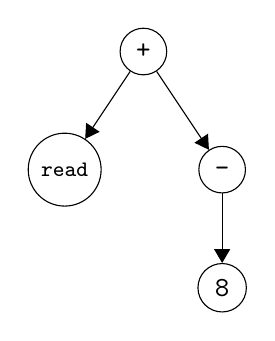
\begin{tikzpicture}
 \node[draw, circle] (plus)  at (0 ,  0) {\key{+}};
 \node[draw, circle] (read)  at (-1, -1.5) {{\footnotesize\key{read}}};
 \node[draw, circle] (minus) at (1 , -1.5) {$\key{-}$};
 \node[draw, circle] (8)     at (1 , -3) {\key{8}};

 \draw[->] (plus) to (read);
 \draw[->] (plus) to (minus);
 \draw[->] (minus) to (8);
\end{tikzpicture}
\label{eq:arith-prog}
\end{equation}
\end{minipage}
\end{center}
We shall use the standard terminology for trees: each circle above is
called a \emph{node}. The arrows connect a node to its \emph{children}
(which are also nodes). The top-most node is the \emph{root}.  Every
node except for the root has a \emph{parent} (the node it is the child
of). If a node has no children, it is a \emph{leaf} node.  Otherwise
it is an \emph{internal} node.

When deciding how to compile the above program, we need to know that
the root node operation is addition and that it has two children:
\texttt{read} and a negation. The abstract syntax tree data structure
directly supports these queries and hence is a good choice. In this
book, we will often write down the textual representation of a program
even when we really have in mind the AST because the textual
representation is more concise.  We recommend that, in your mind, you
alway interpret programs as abstract syntax trees.

\section{Grammars}
\label{sec:grammar}

A programming language can be thought of as a \emph{set} of programs.
The set is typically infinite (one can always create larger and larger
programs), so one cannot simply describe a language by listing all of
the programs in the language. Instead we write down a set of rules, a
\emph{grammar}, for building programs. We shall write our rules in a
variant of Backus-Naur Form (BNF)~\citep{Backus:1960aa,Knuth:1964aa}.
As an example, we describe a small language, named $R_0$, of
integers and arithmetic operations. The first rule says that any
integer is in the language:
\begin{equation}
R_0 ::= \Int  \label{eq:arith-int}
\end{equation}
Each rule has a left-hand-side and a right-hand-side. The way to read
a rule is that if you have all the program parts on the
right-hand-side, then you can create and AST node and categorize it
according to the left-hand-side. (We do not define $\Int$ because the
reader already knows what an integer is.) We make the simplifying
design decision that all of the languages in this book only handle
machine-representable integers (those representable with 64-bits,
i.e., the range $-2^{63}$ to $2^{63}$) which corresponds to the
\texttt{fixnum} datatype in Racket. A name such as $R_0$ that is
defined by the grammar rules is a \emph{non-terminal}.

The second rule for the $R_0$ language is the \texttt{read}
operation that receives an input integer from the user of the program.
\begin{equation}
  R_0 ::= (\key{read}) \label{eq:arith-read}
\end{equation}

The third rule says that, given an $R_0$ node, you can build another
$R_0$ node by negating it.
\begin{equation}
  R_0 ::= (\key{-} \; R_0)  \label{eq:arith-neg}
\end{equation}
Symbols such as \key{-} in typewriter font are \emph{terminal} symbols
and must literally appear in the program for the rule to be
applicable.

We can apply the rules to build ASTs in the $R_0$
language. For example, by rule \eqref{eq:arith-int}, \texttt{8} is an
$R_0$, then by rule \eqref{eq:arith-neg}, the following AST is
an $R_0$.
\begin{center}
\begin{minipage}{0.25\textwidth}
\begin{lstlisting}
(- 8)
\end{lstlisting}
\end{minipage}
\begin{minipage}{0.25\textwidth}
\begin{equation}
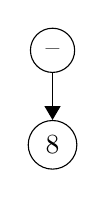
\begin{tikzpicture}
 \node[draw, circle] (minus) at (0, 0)  {$\text{--}$};
 \node[draw, circle] (8)     at (0, -1.2) {$8$};

 \draw[->] (minus) to (8);
\end{tikzpicture}
\label{eq:arith-neg8}
\end{equation}
\end{minipage}
\end{center}

The last rule for the $R_0$ language is for addition:
\begin{equation}
  R_0 ::= (\key{+} \; R_0 \; R_0) \label{eq:arith-add}
\end{equation}
Now we can see that the AST \eqref{eq:arith-prog} is in $R_0$.
We know that \lstinline{(read)} is in $R_0$ by rule
\eqref{eq:arith-read} and we have shown that \texttt{(- 8)} is in
$R_0$, so we can apply rule \eqref{eq:arith-add} to show that
\texttt{(+ (read) (- 8))} is in the $R_0$ language.

If you have an AST for which the above four rules do not apply, then
the AST is not in $R_0$. For example, the AST \texttt{(-
  (read) (+ 8))} is not in $R_0$ because there are no rules
for \key{+} with only one argument, nor for \key{-} with two
arguments.  Whenever we define a language with a grammar, we
implicitly mean for the language to be the smallest set of programs
that are justified by the rules. That is, the language only includes
those programs that the rules allow.

It is common to have many rules with the same left-hand side, so there
is a vertical bar notation for gathering several rules, as shown in
Figure~\ref{fig:r0-syntax}. Each clause between a vertical bar is
called an ``alternative''.

\begin{figure}[tbp]
\fbox{
\begin{minipage}{0.96\textwidth}
\[
R_0 ::= \Int \mid ({\tt \key{read}}) \mid (\key{-} \; R_0) \mid
   (\key{+} \; R_0 \; R_0) 
\]
\end{minipage}
}
\caption{The syntax of the $R_0$ language.}
\label{fig:r0-syntax}
\end{figure}

\section{S-Expressions}
\label{sec:s-expr}

Racket, as a descendant of Lisp, has
convenient support for creating and manipulating abstract syntax trees
with its \emph{symbolic expression} feature, or S-expression for
short. We can create an S-expression simply by writing a backquote
followed by the textual representation of the AST. (Technically
speaking, this is called a \emph{quasiquote} in Racket.)  For example,
an S-expression to represent the AST \eqref{eq:arith-prog} is created
by the following Racket expression:
\begin{center}
\texttt{`(+ (read) (- 8))}
\end{center}

To build larger S-expressions one often needs to splice together
several smaller S-expressions. Racket provides the comma operator to
splice an S-expression into a larger one. For example, instead of
creating the S-expression for AST \eqref{eq:arith-prog} all at once,
we could have first created an S-expression for AST
\eqref{eq:arith-neg8} and then spliced that into the addition
S-expression.
\begin{lstlisting}
   (define ast1.4 `(- 8))
   (define ast1.1 `(+ (read) ,ast1.4))
\end{lstlisting}
In general, the Racket expression that follows the comma (splice)
can be any expression that computes an S-expression.

\section{Pattern Matching}
\label{sec:pattern-matching}

As mentioned above, one of the operations that a compiler needs to
perform on an AST is to access the children of a node.  Racket
provides the \texttt{match} form to access the parts of an
S-expression. Consider the following example and the output on the
right.
\begin{center}
\begin{minipage}{0.5\textwidth}
\begin{lstlisting}
(match ast1.1
  [`(,op ,child1 ,child2)
    (print op) (newline)
    (print child1) (newline)
    (print child2)])
\end{lstlisting}
\end{minipage}
\vrule
\begin{minipage}{0.25\textwidth}
\begin{lstlisting}


   '+
   '(read)
   '(- 8)
\end{lstlisting}
\end{minipage}
\end{center}
The \texttt{match} form takes AST \eqref{eq:arith-prog} and binds its
parts to the three variables \texttt{op}, \texttt{child1}, and
\texttt{child2}. In general, a match clause consists of a
\emph{pattern} and a \emph{body}. The pattern is a quoted S-expression
that may contain pattern-variables (preceded by a comma).  The body
may contain any Racket code.

A \texttt{match} form may contain several clauses, as in the following
function \texttt{leaf?} that recognizes when an $R_0$ node is
a leaf. The \texttt{match} proceeds through the clauses in order,
checking whether the pattern can match the input S-expression. The
body of the first clause that matches is executed. The output of
\texttt{leaf?} for several S-expressions is shown on the right. In the
below \texttt{match}, we see another form of pattern: the \texttt{(?
  fixnum?)} applies the predicate \texttt{fixnum?} to the input
S-expression to see if it is a machine-representable integer.
\begin{center}
\begin{minipage}{0.5\textwidth}
\begin{lstlisting}
(define (leaf? arith)
  (match arith
    [(? fixnum?) #t]
    [`(read) #t]
    [`(- ,c1) #f]
    [`(+ ,c1 ,c2) #f]))

(leaf? `(read))
(leaf? `(- 8))
(leaf? `(+ (read) (- 8)))
\end{lstlisting}
\end{minipage}
\vrule
\begin{minipage}{0.25\textwidth}
\begin{lstlisting}






   #t
   #f
   #f
\end{lstlisting}
\end{minipage}
\end{center}


\section{Recursion}
\label{sec:recursion}

Programs are inherently recursive in that an $R_0$ AST is made
up of smaller $R_0$ ASTs. Thus, the natural way to process in
entire program is with a recursive function.  As a first example of
such a function, we define \texttt{arith?} below, which takes an
arbitrary S-expression, {\tt sexp}, and determines whether or not {\tt
  sexp} is in {\tt arith}. Note that each match clause corresponds to
one grammar rule for $R_0$ and the body of each clause makes a
recursive call for each child node. This pattern of recursive function
is so common that it has a name, \emph{structural recursion}.  In
general, when a recursive function is defined using a sequence of
match clauses that correspond to a grammar, and each clause body makes
a recursive call on each child node, then we say the function is
defined by structural recursion.

\begin{center}
\begin{minipage}{0.7\textwidth}
\begin{lstlisting}
(define (arith? sexp)
  (match sexp
    [(? fixnum?) #t]
    [`(read) #t]
    [`(- ,e) (arith? e)]
    [`(+ ,e1 ,e2)
     (and (arith? e1) (arith? e2))]
    [else #f]))

(arith? `(+ (read) (- 8)))
(arith? `(- (read) (+ 8)))
\end{lstlisting}
\end{minipage}
\vrule
\begin{minipage}{0.25\textwidth}
\begin{lstlisting}








   #t
   #f
\end{lstlisting}
\end{minipage}
\end{center}



\section{Interpreters}
\label{sec:interp-R0}

The meaning, or semantics, of a program is typically defined in the
specification of the language. For example, the Scheme language is
defined in the report by \cite{SPERBER:2009aa}. The Racket language is
defined in its reference manual~\citep{plt-tr}. In this book we use an
interpreter to define the meaning of each language that we consider,
following Reynold's advice in this
regard~\citep{reynolds72:_def_interp}. Here we will warm up by writing
an interpreter for the $R_0$ language, which will also serve
as a second example of structural recursion. The \texttt{interp-R0}
function is defined in Figure~\ref{fig:interp-R0}. The body of the
function is a match on the input expression \texttt{e} and there is
one clause per grammar rule for $R_0$. The clauses for
internal AST nodes make recursive calls to \texttt{interp-R0} on
each child node.

\begin{figure}[tbp]
\begin{lstlisting}
   (define (interp-R0 e)
     (match e
       [(? fixnum?) e]
       [`(read)
        (define r (read))
        (cond [(fixnum? r) r]
              [else (error 'interp-R0 "expected an integer" r)])]
       [`(- ,e)
        (fx- 0 (interp-R0 e))]
       [`(+ ,e1 ,e2)
        (fx+ (interp-R0 e1) (interp-R0 e2))]
       ))
\end{lstlisting}
\caption{Interpreter for the $R_0$ language.}
\label{fig:interp-R0}
\end{figure}

Let us consider the result of interpreting some example $R_0$
programs. The following program simply adds two integers.
\begin{lstlisting}
   (+ 10 32)
\end{lstlisting}
The result is \key{42}, as you might expected. 
%
The next example demonstrates that expressions may be nested within
each other, in this case nesting several additions and negations.
\begin{lstlisting}
   (+ 10 (- (+ 12 20)))
\end{lstlisting}
What is the result of the above program?

If we interpret the AST \eqref{eq:arith-prog} and give it the input
\texttt{50}
\begin{lstlisting}
   (interp-R0 ast1.1)
\end{lstlisting}
we get the answer to life, the universe, and everything:
\begin{lstlisting}
   42
\end{lstlisting}

Moving on, the \key{read} operation prompts the user of the program
for an integer. Given an input of \key{10}, the following program
produces \key{42}.
\begin{lstlisting}
   (+ (read) 32)
\end{lstlisting}
We include the \key{read} operation in $R_1$ so that a compiler for
$R_1$ cannot be implemented simply by running the interpreter at
compilation time to obtain the output and then generating the trivial
code to return the output. (A clever student at Colorado did this the
first time I taught the course.)

%% The behavior of the following program is somewhat subtle because
%% Racket does not specify an evaluation order for arguments of an
%% operator such as $-$.
%% \marginpar{\scriptsize This is not true of Racket. \\ --Jeremy}
%% \[
%% \BINOP{+}{\READ}{\UNIOP{-}{\READ}}
%% \]
%% Given the input $42$ then $10$, the above program can result in either
%% $42$ or $-42$, depending on the whims of the Racket implementation.

The job of a compiler is to translate a program in one language into a
program in another language so that the output program behaves the
same way as the input program. This idea is depicted in the following
diagram. Suppose we have two languages, $\mathcal{L}_1$ and
$\mathcal{L}_2$, and an interpreter for each language.  Suppose that
the compiler translates program $P_1$ in language $\mathcal{L}_1$ into
program $P_2$ in language $\mathcal{L}_2$.  Then interpreting $P_1$
and $P_2$ on their respective interpreters with input $i$ should yield
the same output $o$.
\begin{equation} \label{eq:compile-correct}
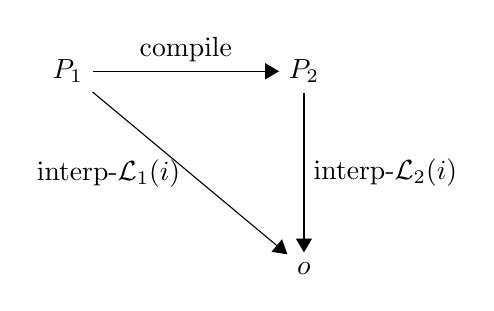
\begin{tikzpicture}[baseline=(current  bounding  box.center)]
 \node (p1) at (0,  0) {$P_1$};
 \node (p2) at (3,  0) {$P_2$};
 \node (o)  at (3, -2.5) {$o$};

 \path[->] (p1) edge [above] node {compile} (p2);
 \path[->] (p2) edge [right] node {interp-$\mathcal{L}_2$($i$)} (o);
 \path[->] (p1) edge [left]  node {interp-$\mathcal{L}_1$($i$)} (o);
\end{tikzpicture}
\end{equation}
In the next section we see our first example of a compiler, which is
another example of structural recursion.


\section{Partial Evaluation}
\label{sec:partial-evaluation}

In this section we consider a compiler that translates $R_0$
programs into $R_0$ programs that are more efficient, that is,
this compiler is an optimizer. Our optimizer will accomplish this by
trying to eagerly compute the parts of the program that do not depend
on any inputs. For example, given the following program
\begin{lstlisting}
   (+ (read) (- (+ 5 3)))
\end{lstlisting}
our compiler will translate it into the program
\begin{lstlisting}
   (+ (read) -8)
\end{lstlisting}

Figure~\ref{fig:pe-arith} gives the code for a simple partial
evaluator for the $R_0$ language. The output of the partial
evaluator is an $R_0$ program, which we build up using a
combination of quasiquotes and commas. (Though no quasiquote is
necessary for integers.) In Figure~\ref{fig:pe-arith}, the normal
structural recursion is captured in the main \texttt{pe-arith}
function whereas the code for partially evaluating negation and
addition is factored out the into two separate helper functions:
\texttt{pe-neg} and \texttt{pe-add}. The input to these helper
functions is the output of partially evaluating the children nodes.

\begin{figure}[tbp]
\begin{lstlisting}
   (define (pe-neg r)
     (match r
       [(? fixnum?) (fx- 0 r)]
       [else `(- ,r)]))
   (define (pe-add r1 r2)
     (match (list r1 r2)
       [`(,n1 ,n2) #:when (and (fixnum? n1) (fixnum? n2))
        (fx+ r1 r2)]
       [else `(+ ,r1 ,r2)]))
   (define (pe-arith e)
     (match e
       [(? fixnum?) e]
       [`(read) `(read)]
       [`(- ,e1) (pe-neg (pe-arith e1))]
       [`(+ ,e1 ,e2) (pe-add (pe-arith e1) (pe-arith e2))]))   
\end{lstlisting}
\caption{A partial evaluator for the $R_0$ language.}
\label{fig:pe-arith}
\end{figure}

Our code for \texttt{pe-neg} and \texttt{pe-add} implements the simple
idea of checking whether the inputs are integers and if they are, to
go ahead perform the arithmetic.  Otherwise, we use quasiquote to
create an AST node for the appropriate operation (either negation or
addition) and use comma to splice in the child nodes.

To gain some confidence that the partial evaluator is correct, we can
test whether it produces programs that get the same result as the
input program. That is, we can test whether it satisfies Diagram
\eqref{eq:compile-correct}. The following code runs the partial
evaluator on several examples and tests the output program.  The
\texttt{assert} function is defined in Appendix~\ref{appendix:utilities}.
\begin{lstlisting}
(define (test-pe pe p)
  (assert "testing pe-arith"
     (equal? (interp-R0 p) (interp-R0 (pe-arith p)))))

(test-pe `(+ (read) (- (+ 5 3))))
(test-pe `(+ 1 (+ (read) 1)))
(test-pe `(- (+ (read) (- 5))))
\end{lstlisting}

\begin{exercise}
\normalfont % I don't like the italics for exercises. -Jeremy
We challenge the reader to improve on the simple partial evaluator in
Figure~\ref{fig:pe-arith} by replacing the \texttt{pe-neg} and
\texttt{pe-add} helper functions with functions that know more about
arithmetic. For example, your partial evaluator should translate
\begin{lstlisting}
   (+ 1 (+ (read) 1))
\end{lstlisting}
into
\begin{lstlisting}
   (+ 2 (read))
\end{lstlisting}
To accomplish this, we recommend that your partial evaluator produce
output that takes the form of the $\itm{residual}$ non-terminal in the
following grammar.
\[
\begin{array}{lcl}
\Exp &::=& (\key{read}) \mid (\key{-} \;(\key{read})) \mid (\key{+} \; \Exp \; \Exp)\\
\itm{residual} &::=& \Int \mid (\key{+}\; \Int\; \Exp) \mid \Exp
\end{array}
\]
\end{exercise}


%%%%%%%%%%%%%%%%%%%%%%%%%%%%%%%%%%%%%%%%%%%%%%%%%%%%%%%%%%%%%%%%%%%%%%%%%%%%%%%%
\chapter{Compiling Integers and Variables}
\label{ch:int-exp}

This chapter concerns the challenge of compiling a subset of Racket,
which we name $R_1$, to x86-64 assembly code~\citep{Matz:2013aa}. The
chapter begins with a description of the $R_1$ language
(Section~\ref{sec:s0}) and then a description of x86-64
(Section~\ref{sec:x86-64}). The x86-64 assembly language is quite
large, so we only discuss what is needed for compiling $R_1$. We
introduce more of x86-64 in later chapters. Once we have introduced
$R_1$ and x86-64, we reflect on their differences and come up with a
plan breaking down the translation from $R_1$ to x86-64 into a handful
of steps (Section~\ref{sec:plan-s0-x86}).  The rest of the sections in
this Chapter give detailed hints regarding each step
(Sections~\ref{sec:uniquify-s0} through \ref{sec:patch-s0}).  We hope
to give enough hints that the well-prepared reader can implement a
compiler from $R_1$ to x86-64 while at the same time leaving room for
some fun and creativity.

\section{The $R_1$ Language}
\label{sec:s0}

The $R_1$ language extends the $R_0$ language
(Figure~\ref{fig:r0-syntax}) with variable definitions.  The syntax of
the $R_1$ language is defined by the grammar in
Figure~\ref{fig:r1-syntax}. As in $R_0$, \key{read} is a nullary
operator, \key{-} is a unary operator, and \key{+} is a binary
operator. In addition to variable definitions, the $R_1$ language
includes the \key{program} form to mark the top of the program, which
is helpful in some of the compiler passes.  The $R_1$ language is rich
enough to exhibit several compilation techniques but simple enough so
that the reader can implement a compiler for it in a week of part-time
work.  To give the reader a feeling for the scale of this first
compiler, the instructor solution for the $R_1$ compiler consists of 6
recursive functions and a few small helper functions that together
span 256 lines of code.

\begin{figure}[btp]
\centering
\fbox{
\begin{minipage}{0.96\textwidth}
\[
\begin{array}{rcl}
\Op  &::=& \key{read} \mid \key{-} \mid \key{+} \\
\Exp &::=& \Int \mid (\Op \; \Exp^{*})  \mid  \Var \mid \LET{\Var}{\Exp}{\Exp} \\
R_1  &::=& (\key{program} \; \Exp)
\end{array}
\]
\end{minipage}
}
\caption{The syntax of the $R_1$ language. 
  The non-terminal \Var{} may be any Racket identifier.}
\label{fig:r1-syntax}
\end{figure}

The \key{let} construct defines a variable for use within its body
and initializes the variable with the value of an expression.  So the
following program initializes \code{x} to \code{32} and then evaluates
the body \code{(+ 10 x)}, producing \code{42}.
\begin{lstlisting}
   (program
      (let ([x (+ 12 20)]) (+ 10 x)))
\end{lstlisting}
When there are multiple \key{let}'s for the same variable, the closest
enclosing \key{let} is used. That is, variable definitions overshadow
prior definitions. Consider the following program with two \key{let}'s
that define variables named \code{x}. Can you figure out the result?
\begin{lstlisting}
   (program
      (let ([x 32]) (+ (let ([x 10]) x) x)))
\end{lstlisting}
For the purposes of showing which variable uses correspond to which
definitions, the following shows the \code{x}'s annotated with subscripts
to distinguish them. Double check that your answer for the above is
the same as your answer for this annotated version of the program.
\begin{lstlisting}
   (program
      (let ([x|$_1$| 32]) (+ (let ([x|$_2$| 10]) x|$_2$|) x|$_1$|)))
\end{lstlisting}
The initializing expression is always evaluated before the body of the
\key{let}, so in the following, the \key{read} for \code{x} is
performed before the \key{read} for \code{y}. Given the input
\code{52} then \code{10}, the following produces \code{42} (and not
\code{-42}).
\begin{lstlisting}
   (program
     (let ([x (read)]) (let ([y (read)]) (- x y))))
\end{lstlisting}

Figure~\ref{fig:interp-R1} shows the interpreter for the $R_1$
language. It extends the interpreter for $R_0$ with two new
\key{match} clauses for variables and for \key{let}.  For \key{let},
we will need a way to communicate the initializing value of a variable
to all the uses of a variable. To accomplish this, we maintain a
mapping from variables to values, which is traditionally called an
\emph{environment}. For simplicity, here we use an association list to
represent the environment. The \code{interp-R1} function takes the
current environment, \code{env}, as an extra parameter.  When the
interpreter encounters a variable, it finds the corresponding value
using the \code{lookup} function (Appendix~\ref{appendix:utilities}).
When the interpreter encounters a \key{let}, it evaluates the
initializing expression, extends the environment with the result bound
to the variable, then evaluates the body of the \key{let}.

\begin{figure}[tbp]
\begin{lstlisting}
   (define (interp-R1 env e)
     (match e
       [(? symbol?) (lookup e env)]
       [`(let ([,x ,e]) ,body)
        (define v (interp-R1 env e))
        (define new-env (cons (cons x v) env))
        (interp-R1 new-env body)]
       [(? fixnum?) e]
       [`(read)
        (define r (read))
        (cond [(fixnum? r) r]
              [else (error 'interp-R1 "expected an integer" r)])]
       [`(- ,e)
        (fx- 0 (interp-R1 env e))]
       [`(+ ,e1 ,e2)
        (fx+ (interp-R1 env e1) (interp-R1 env e2))]
       [`(program ,e) (interp-R1 '() e)]
       ))
\end{lstlisting}
\caption{Interpreter for the $R_1$ language.}
\label{fig:interp-R1}
\end{figure}



The goal for this chapter is to implement a compiler that translates
any program $P_1$ in the $R_1$ language into an x86-64 assembly
program $P_2$ such that $P_2$ exhibits the same behavior on an x86
computer as the $R_1$ program running in a Racket implementation.
That is, they both output the same integer $n$.
\[
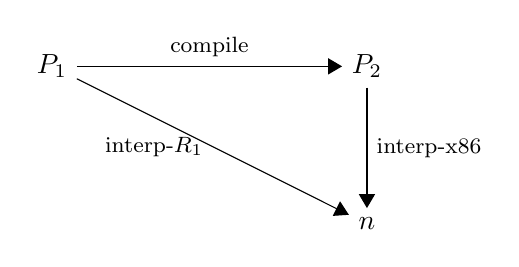
\begin{tikzpicture}[baseline=(current  bounding  box.center)]
 \node (p1) at (0,  0)   {$P_1$};
 \node (p2) at (4,  0)   {$P_2$};
 \node (o)  at (4, -2) {$n$};

 \path[->] (p1) edge [above] node {\footnotesize compile} (p2);
 \path[->] (p1) edge [left]  node {\footnotesize interp-$R_1$} (o);
 \path[->] (p2) edge [right] node {\footnotesize interp-x86} (o);
\end{tikzpicture}
\]
In the next section we introduce enough of the x86-64 assembly
language to compile $R_1$.

\section{The x86-64 Assembly Language}
\label{sec:x86-64}

An x86-64 program is a sequence of instructions. The instructions may
refer to integer constants (called \emph{immediate values}), variables
called \emph{registers}, and instructions may load and store values
into \emph{memory}.  Memory is a mapping of 64-bit addresses to 64-bit
values. Figure~\ref{fig:x86-a} defines the syntax for the subset of
the x86-64 assembly language needed for this chapter.  (We use the
AT\&T syntax expected by the GNU assembler inside \key{gcc}.)

An immediate value is written using the notation \key{\$}$n$ where $n$
is an integer. 
%
A register is written with a \key{\%} followed by the register name,
such as \key{\%rax}.
%
An access to memory is specified using the syntax $n(\key{\%}r)$,
which reads register $r$ and then offsets the address by $n$ bytes (8
bits). The address is then used to either load or store to memory
depending on whether it occurs as a source or destination argument of
an instruction.

An arithmetic instruction, such as $\key{addq}\,s,\,d$, reads from the
source $s$ and destination $d$, applies the arithmetic operation, then
write the result in $d$.
%
The move instruction, $\key{movq}\,s\,d$ reads from $s$ and stores the
result in $d$. 
%
The $\key{callq}\,\mathit{label}$ instruction executes the procedure
specified by the label.

\begin{figure}[tbp]
\fbox{
\begin{minipage}{0.96\textwidth}
\[
\begin{array}{lcl}
\Reg &::=& \key{rsp} \mid \key{rbp} \mid \key{rax} \mid \key{rbx} \mid \key{rcx}
              \mid \key{rdx} \mid \key{rsi} \mid \key{rdi} \mid \\
              && \key{r8} \mid \key{r9} \mid \key{r10}
              \mid \key{r11} \mid \key{r12} \mid \key{r13}
              \mid \key{r14} \mid \key{r15} \\
\Arg &::=&  \key{\$}\Int \mid \key{\%}\Reg \mid \Int(\key{\%}\Reg) \\ 
\Instr &::=& \key{addq} \; \Arg, \Arg \mid 
      \key{subq} \; \Arg, \Arg \mid 
%      \key{imulq} \; \Arg,\Arg \mid 
      \key{negq} \; \Arg \mid \key{movq} \; \Arg, \Arg \mid \\
  &&  \key{callq} \; \mathit{label} \mid
      \key{pushq}\;\Arg \mid \key{popq}\;\Arg \mid \key{retq} \\
\Prog &::= & \key{.globl \_main}\\
      &    & \key{\_main:} \; \Instr^{+}
\end{array}
\]
\end{minipage}
}
\caption{A subset of the x86-64 assembly language (AT\&T syntax).}
\label{fig:x86-a}
\end{figure}


\begin{wrapfigure}{r}{2.25in}
\begin{lstlisting}
	.globl _main
_main:
	movq	$10, %rax
	addq	$32, %rax
	retq
\end{lstlisting}
\caption{An x86-64 program equivalent to $\BINOP{+}{10}{32}$.}
\label{fig:p0-x86}
\end{wrapfigure}

Figure~\ref{fig:p0-x86} depicts an x86-64 program that is equivalent
to \code{(+ 10 32)}. The \key{globl} directive says that the
\key{\_main} procedure is externally visible, which is necessary so
that the operating system can call it. The label \key{\_main:}
indicates the beginning of the \key{\_main} procedure which is where
the operating system starting executing this program.  The instruction
\lstinline{movq $10, %rax} puts $10$ into register \key{rax}. The
following instruction \lstinline{addq $32, %rax} adds $32$ to the
$10$ in \key{rax} and puts the result, $42$, back into
\key{rax}. The instruction \key{retq} finishes the \key{\_main}
function by returning the integer in \key{rax} to the
operating system.


\begin{wrapfigure}{r}{2.25in}
\begin{lstlisting}
	.globl _main
_main:
	pushq	%rbp
	movq	%rsp, %rbp
	subq	$16, %rsp

	movq	$10, -8(%rbp)
	negq	-8(%rbp)
	movq	$52, %rax
	addq	-8(%rbp), %rax

	addq	$16, %rsp
	popq	%rbp
	retq
\end{lstlisting}
\caption{An x86-64 program equivalent to $\BINOP{+}{52}{\UNIOP{-}{10} }$.}
\label{fig:p1-x86}
\end{wrapfigure}

The next example exhibits the use of memory.  Figure~\ref{fig:p1-x86}
lists an x86-64 program that is equivalent to $\BINOP{+}{52}{
  \UNIOP{-}{10} }$. To understand how this x86-64 program works, we
need to explain a region of memory called called the \emph{procedure
  call stack} (or \emph{stack} for short). The stack consists of a
separate \emph{frame} for each procedure call. The memory layout for
an individual frame is shown in Figure~\ref{fig:frame}.  The register
\key{rsp} is called the \emph{stack pointer} and points to the item at
the top of the stack. The stack grows downward in memory, so we
increase the size of the stack by subtracting from the stack
pointer. The frame size is required to be a multiple of 16 bytes. The
register \key{rbp} is the \emph{base pointer} which serves two
purposes: 1) it saves the location of the stack pointer for the
procedure that called the current one and 2) it is used to access
variables associated with the current procedure. We number the
variables from $1$ to $n$. Variable $1$ is stored at address
$-8\key{(\%rbp)}$, variable $2$ at $-16\key{(\%rbp)}$, etc.

\begin{figure}[tbp]
\centering
\begin{tabular}{|r|l|} \hline
Position & Contents \\ \hline
8(\key{\%rbp}) & return address \\
0(\key{\%rbp}) & old \key{rbp} \\
-8(\key{\%rbp}) & variable $1$ \\
-16(\key{\%rbp}) & variable $2$ \\
 \ldots  & \ldots \\
0(\key{\%rsp}) & variable $n$\\ \hline
\end{tabular}

\caption{Memory layout of a frame.}
\label{fig:frame}
\end{figure}

Getting back to the program in Figure~\ref{fig:p1-x86}, the first
three instructions are the typical prelude for a procedure.  The
instruction \key{pushq \%rbp} saves the base pointer for the procedure
that called the current one onto the stack and subtracts $8$ from the
stack pointer. The second instruction \key{movq \%rsp, \%rbp} changes
the base pointer to the top of the stack. The instruction \key{subq
  \$16, \%rsp} moves the stack pointer down to make enough room for
storing variables.  This program just needs one variable ($8$ bytes)
but because the frame size is required to be a multiple of 16 bytes,
it rounds to 16 bytes.

The next four instructions carry out the work of computing
$\BINOP{+}{52}{\UNIOP{-}{10} }$. The first instruction \key{movq \$10,
  -8(\%rbp)} stores $10$ in variable $1$. The instruction \key{negq
  -8(\%rbp)} changes variable $1$ to $-10$. The \key{movq \$52, \%rax}
places $52$ in the register \key{rax} and \key{addq -8(\%rbp), \%rax}
adds the contents of variable $1$ to \key{rax}, at which point
\key{rax} contains $42$.

The last three instructions are the typical \emph{conclusion} of a
procedure. These instructions are necessary to get the state of the
machine back to where it was before the current procedure was called.
The \key{addq \$16, \%rsp} instruction moves the stack pointer back to
point at the old base pointer. The amount added here needs to match
the amount that was subtracted in the prelude of the procedure.  Then
\key{popq \%rbp} returns the old base pointer to \key{rbp} and adds
$8$ to the stack pointer.  The \key{retq} instruction jumps back to
the procedure that called this one and subtracts 8 from the stack
pointer.

The compiler will need a convenient representation for manipulating
x86 programs, so we define an abstract syntax for x86 in
Figure~\ref{fig:x86-ast-a}. The \itm{info} field of the \key{program}
AST node is for storing auxilliary information that needs to be
communicated from one step of the compiler to the next. 

\begin{figure}[tbp]
\fbox{
\begin{minipage}{0.96\textwidth}
\[
\begin{array}{lcl}
\Arg &::=&  \INT{\Int} \mid \REG{\itm{register}}
    \mid \STACKLOC{\Int} \\ 
\Instr &::=& (\key{addq} \; \Arg\; \Arg) \mid 
             (\key{subq} \; \Arg\; \Arg) \mid 
%             (\key{imulq} \; \Arg\;\Arg) \mid 
             (\key{negq} \; \Arg) \mid (\key{movq} \; \Arg\; \Arg) \\
      &\mid& (\key{callq} \; \mathit{label}) \mid
             (\key{pushq}\;\Arg) \mid 
             (\key{popq}\;\Arg) \mid 
             (\key{retq}) \\
\Prog &::= & (\key{program} \;\itm{info} \; \Instr^{+})
\end{array}
\]
\end{minipage}
}
\caption{Abstract syntax for x86-64 assembly.}
\label{fig:x86-ast-a}
\end{figure}

\section{Planning the trip from $R_1$ to x86-64}
\label{sec:plan-s0-x86}

To compile one language to another it helps to focus on the
differences between the two languages. It is these differences that
the compiler will need to bridge. What are the differences between
$R_1$ and x86-64 assembly? Here we list some of the most important the
differences.

\begin{enumerate}
\item x86-64 arithmetic instructions typically take two arguments and
  update the second argument in place. In contrast, $R_1$ arithmetic
  operations only read their arguments and produce a new value.

\item An argument to an $R_1$ operator can be any expression, whereas
  x86-64 instructions restrict their arguments to integers, registers,
  and memory locations.

\item An $R_1$ program can have any number of variables whereas x86-64
  has only 16 registers.

\item Variables in $R_1$ can overshadow other variables with the same
  name. The registers and memory locations of x86-64 all have unique
  names.
\end{enumerate}

We ease the challenge of compiling from $R_1$ to x86 by breaking down
the problem into several steps, dealing with the above differences one
at a time. The main question then becomes: in what order do we tackle
these differences? This is often one of the most challenging questions
that a compiler writer must answer because some orderings may be much
more difficult to implement than others. It is difficult to know ahead
of time which orders will be better so often some trial-and-error is
involved. However, we can try to plan ahead and choose the orderings
based on this planning.

For example, to handle difference \#2 (nested expressions), we shall
introduce new variables and pull apart the nested expressions into a
sequence of assignment statements.  To deal with difference \#3 we
will be replacing variables with registers and/or stack
locations. Thus, it makes sense to deal with \#2 before \#3 so that
\#3 can replace both the original variables and the new ones. Next,
consider where \#1 should fit in. Because it has to do with the format
of x86 instructions, it makes more sense after we have flattened the
nested expressions (\#2). Finally, when should we deal with \#4
(variable overshadowing)?  We shall solve this problem by renaming
variables to make sure they have unique names. Recall that our plan
for \#2 involves moving nested expressions, which could be problematic
if it changes the shadowing of variables. However, if we deal with \#4
first, then it will not be an issue.  Thus, we arrive at the following
ordering.
\[
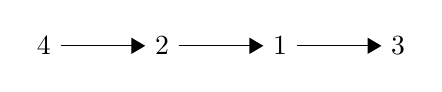
\begin{tikzpicture}[baseline=(current  bounding  box.center)]
\foreach \i/\p in {4/1,2/2,1/3,3/4}
{ 
  \node (\i) at (\p*1.5,0) {$\i$};
}
\foreach \x/\y in {4/2,2/1,1/3}
{
  \draw[->] (\x) to (\y);
}
\end{tikzpicture}
\]
We further simplify the translation from $R_1$ to x86 by identifying
an intermediate language named $C_0$, roughly half-way between $R_1$
and x86, to provide a rest stop along the way. We name the language
$C_0$ because it is vaguely similar to the $C$
language~\citep{Kernighan:1988nx}. The differences \#4 and \#1,
regarding variables and nested expressions, will be handled by two
steps, \key{uniquify} and \key{flatten}, which bring us to
$C_0$.
\[
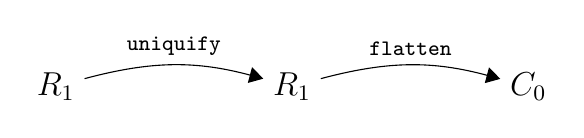
\begin{tikzpicture}[baseline=(current  bounding  box.center)]
\foreach \i/\p in {R_1/1,R_1/2,C_0/3}
{ 
  \node (\p) at (\p*3,0) {\large $\i$};
}
\foreach \x/\y/\lbl in {1/2/uniquify,2/3/flatten}
{
 \path[->,bend left=15] (\x) edge [above] node {\ttfamily\footnotesize \lbl} (\y);
}
\end{tikzpicture}
\]
Each of these steps in the compiler is implemented by a function,
typically a structurally recursive function that translates an input
AST into an output AST. We refer to such a function as a \emph{pass}
because it makes a pass over, i.e. traverses, the entire AST.

The syntax for $C_0$ is defined in Figure~\ref{fig:c0-syntax}.  The
$C_0$ language supports the same operators as $R_1$ but the arguments
of operators are now restricted to just variables and integers. The
\key{let} construct of $R_1$ is replaced by an assignment statement
and there is a \key{return} construct to specify the return value of
the program. A program consists of a sequence of statements that
include at least one \key{return} statement. Each program is also
annotated with a list of variables. At the start of the program, these
variables are uninitialized (they contain garbage) and each variable
becomes initialized on its first assignment. All of the variables used
in the program must be present in this list.

\begin{figure}[tbp]
\fbox{
\begin{minipage}{0.96\textwidth}
\[
\begin{array}{lcl}
\Arg &::=& \Int \mid \Var \\
\Exp &::=& \Arg \mid (\Op \; \Arg^{*})\\
\Stmt &::=& \ASSIGN{\Var}{\Exp} \mid \RETURN{\Arg} \\
\Prog & ::= & (\key{program}\;(\Var^{*})\;\Stmt^{+})
\end{array}
\]
\end{minipage}
}
\caption{The $C_0$ intermediate language.}
\label{fig:c0-syntax}
\end{figure}

To get from $C_0$ to x86-64 assembly it remains for us to handle
difference \#1 (the format of instructions) and difference \#3
(variables versus registers). These two differences are intertwined,
creating a bit of a Gordian Knot. To handle difference \#3, we need to
map some variables to registers (there are only 16 registers) and the
remaining variables to locations on the stack (which is unbounded). To
make good decisions regarding this mapping, we need the program to be
close to its final form (in x86-64 assembly) so we know exactly when
which variables are used. After all, variables that are used in
disjoint parts of the program can be assigned to the same register.
However, our choice of x86-64 instructions depends on whether the
variables are mapped to registers or stack locations, so we have a
circular dependency. We cut this knot by doing an optimistic selection
of instructions in the \key{select-instructions} pass, followed by the
\key{assign-homes} pass to map variables to registers or stack
locations, and conclude by finalizing the instruction selection in the
\key{patch-instructions} pass.
\[
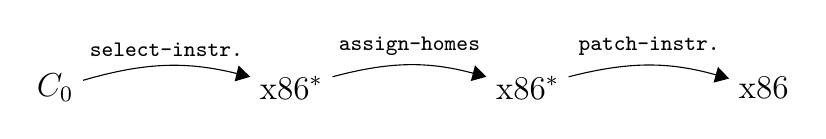
\begin{tikzpicture}[baseline=(current  bounding  box.center)]
\node (1) at (0,0)  {\large $C_0$};
\node (2) at (3,0)  {\large $\text{x86}^{*}$};
\node (3) at (6,0)  {\large $\text{x86}^{*}$};
\node (4) at (9,0) {\large $\text{x86}$};

\path[->,bend left=15] (1) edge [above] node {\ttfamily\footnotesize select-instr.} (2);
\path[->,bend left=15] (2) edge [above] node {\ttfamily\footnotesize assign-homes} (3);
\path[->,bend left=15] (3) edge [above] node {\ttfamily\footnotesize patch-instr.} (4);
\end{tikzpicture}
\]

The \key{select-instructions} pass is optimistic in the sense that it
treats variables as if they were all mapped to registers. The
\key{select-instructions} pass generates a program that consists of
x86-64 instructions but that still use variables, so it is an
intermediate language that is technically different than x86-64, which
explains the astericks in the diagram above.

In this Chapter we shall take the easy road to implementing
\key{assign-homes} and simply map all variables to stack locations.
The topic of Chapter~\ref{ch:register-allocation} is implementing a
smarter approach in which we make a best-effort to map variables to
registers, resorting to the stack only when necessary.

%% \marginpar{\scriptsize I'm confused: shouldn't `select instructions' do this?
%% After all, that selects the x86-64 instructions. Even if it is separate,
%% if we perform `patching' before register allocation, we aren't forced to rely on
%% \key{rax} as much. This can ultimately make a more-performant result. --
%% Cam}


Once variables have been assigned to their homes, we can finalize the
instruction selection by dealing with an indiosycracy of x86
assembly. Many x86 instructions have two arguments but only one of the
arguments may be a memory reference (and the stack is a part of
memory).  Because some variables may get mapped to stack locations,
some of our generated instructions may violate this restriction.  The
purpose of the \key{patch-instructions} pass is to fix this problem by
replacing every violating instruction with a short sequence of
instructions that use the \key{rax} register. Once we have implemented
a good register allocator (Chapter~\ref{ch:register-allocation}), the
need to patch instructions will be relatively rare.


\section{Uniquify Variables}
\label{sec:uniquify-s0}

The purpose of this pass is to make sure that each \key{let} uses a
unique variable name. For example, the \code{uniquify} pass should
translate the program on the left into the program on the right. \\
\begin{tabular}{lll}
\begin{minipage}{0.4\textwidth}
\begin{lstlisting}
 (program
   (let ([x 32])
     (+ (let ([x 10]) x) x)))
\end{lstlisting}
\end{minipage}
&
$\Rightarrow$
&
\begin{minipage}{0.4\textwidth}
\begin{lstlisting}
(program
  (let ([x.1 32])
    (+ (let ([x.2 10]) x.2) x.1)))
\end{lstlisting}
\end{minipage}
\end{tabular} \\
%
The following is another example translation, this time of a program
with a \key{let} nested inside the initializing expression of another
\key{let}.\\
\begin{tabular}{lll}
\begin{minipage}{0.4\textwidth}
\begin{lstlisting}
(program
  (let ([x (let ([x 4])
             (+ x 1))])
    (+ x 2)))
\end{lstlisting}
\end{minipage}
&
$\Rightarrow$
&
\begin{minipage}{0.4\textwidth}
\begin{lstlisting}
(program
  (let ([x.2 (let ([x.1 4])
               (+ x.1 1))])
    (+ x.2 2)))
\end{lstlisting}
\end{minipage}
\end{tabular}

We recommend implementing \code{uniquify} as a structurally recursive
function that mostly copies the input program. However, when
encountering a \key{let}, it should generate a unique name for the
variable (the Racket function \code{gensym} is handy for this) and
associate the old name with the new unique name in an association
list. The \code{uniquify} function will need to access this
association list when it gets to a variable reference, so we add
another parameter to \code{uniquify} for the association list. It is
quite common for a compiler pass to need a map to store extra
information about variables. Such maps are often called \emph{symbol
  tables}.

The skeleton of the \code{uniquify} function is shown in
Figure~\ref{fig:uniquify-s0}.  The function is curried so that it is
convenient to partially apply it to an association list and then apply
it to different expressions, as in the last clause for primitive
operations in Figure~\ref{fig:uniquify-s0}. In the last \key{match}
clause for the primitive operators, note the use of the comma-@
operator to splice a list of S-expressions into an enclosing
S-expression.

\begin{exercise}
\normalfont % I don't like the italics for exercises. -Jeremy

Complete the \code{uniquify} pass by filling in the blanks, that is,
implement the clauses for variables and for the \key{let} construct.
\end{exercise}

\begin{figure}[tbp]
\begin{lstlisting}
   (define uniquify
     (lambda (alist)
       (lambda (e)
         (match e
           [(? symbol?) ___]
           [(? integer?) e]
           [`(let ([,x ,e]) ,body) ___]
           [`(program ,e)
            `(program ,((uniquify alist) e))]
           [`(,op ,es ...)
            `(,op ,@(map (uniquify alist) es))]
           ))))
\end{lstlisting}
\caption{Skeleton for the \key{uniquify} pass.}
\label{fig:uniquify-s0}
\end{figure}

\begin{exercise}
\normalfont % I don't like the italics for exercises. -Jeremy 

Test your \key{uniquify} pass by creating five example $R_1$ programs
and checking whether the output programs produce the same result as
the input programs. The $R_1$ programs should be designed to test the
most interesting parts of the \key{uniquify} pass, that is, the
programs should include \key{let} constructs, variables, and variables
that overshadow each other.  The five programs should be in a
subdirectory named \key{tests} and they should have the same file name
except for a different integer at the end of the name, followed by the
ending \key{.scm}.  Use the \key{interp-tests} function
(Appendix~\ref{appendix:utilities}) from \key{utilities.rkt} to test
your \key{uniquify} pass on the example programs.

%% You can use the interpreter \key{interpret-S0} defined in the
%% \key{interp.rkt} file. The entire sequence of tests should be a short
%% Racket program so you can re-run all the tests by running the Racket
%% program. We refer to this as the \emph{regression test} program.
\end{exercise}


\section{Flatten Expressions}
\label{sec:flatten-s0}

The \code{flatten} pass will transform $R_1$ programs into $C_0$
programs. In particular, the purpose of the \code{flatten} pass is to
get rid of nested expressions, such as the \code{(- 10)} in the below
program. This can be accomplished by introducing a new variable,
assigning the nested expression to the new variable, and then using
the new variable in place of the nested expressions, as shown in the
output of \code{flatten} on the right.\\
\begin{tabular}{lll}
\begin{minipage}{0.4\textwidth}
\begin{lstlisting}
 (program
   (+ 52 (- 10)))
\end{lstlisting}
\end{minipage}
&
$\Rightarrow$
&
\begin{minipage}{0.4\textwidth}
\begin{lstlisting}
(program (tmp.1 tmp.2)
  (assign tmp.1 (- 10))
  (assign tmp.2 (+ 52 tmp.1))
  (return tmp.2))
\end{lstlisting}
\end{minipage}
\end{tabular}

The clause of \code{flatten} for \key{let} is straightforward to
implement as it just requires the generation of an assignment
statement for the \key{let}-bound variable. The following shows the
result of \code{flatten} for a \key{let}. \\
\begin{tabular}{lll}
\begin{minipage}{0.4\textwidth}
\begin{lstlisting}
 (program
   (let ([x (+ (- 10) 11)])
     (+ x 41)))
\end{lstlisting}
\end{minipage}
&
$\Rightarrow$
&
\begin{minipage}{0.4\textwidth}
\begin{lstlisting}
(program (tmp.1 x tmp.2)
  (assign tmp.1 (- 10))
  (assign x (+ tmp.1 11))
  (assign tmp.2 (+ x 41))
  (return tmp.2))
\end{lstlisting}
\end{minipage}
\end{tabular}

We recommend implementing \key{flatten} as a structurally recursive
function that returns two things, 1) the newly flattened expression,
and 2) a list of assignment statements, one for each of the new
variables introduced while flattening the expression.  The newly
flattened expression should be leaf node. You can return multiple
things from a function using the \key{values} form and you can receive
multiple things from a function call using the \key{define-values}
form. If you are not familiar with these constructs, the Racket
documentation will be of help. Also, the \key{map2} function
(Appendix~\ref{appendix:utilities}) is useful for applying a function
to each element of a list, in the case where the function returns two
values. The result of \key{map2} is two lists.

The clause of \key{flatten} for the \key{program} node needs to
recursively flatten the body of the program and also compute the list
of variables used in the program.  I recommend traversing the
statements in the body of the program (after it has been flattened)
and collect all variables that appear on the left-hand-side of an
assignment. Note that each variable should only occur ones in the list
of variables that you place in the \key{program} form.

Take special care for programs such as the following that initialize
variables with integers or other variables. It should be translated
to the program on the right \\
\begin{tabular}{lll}
\begin{minipage}{0.4\textwidth}
\begin{lstlisting}
  (let ([a 42])
    (let ([b a])
      b))
\end{lstlisting}
\end{minipage}
&
$\Rightarrow$
&
\begin{minipage}{0.4\textwidth}
\begin{lstlisting}
(program (a b)
  (assign a 42)
  (assign b a)
  (return b))
\end{lstlisting}
\end{minipage}
\end{tabular} \\
and not to the following, which could result from a naive
implementation of \key{flatten}.
\begin{lstlisting}
   (program (tmp.1 a tmp.2 b)
     (assign tmp.1 42)
     (assign a tmp.1)
     (assign tmp.2 a)
     (assign b tmp.2)
     (return b))
\end{lstlisting}

\begin{exercise}
\normalfont
Implement the \key{flatten} pass and test it on all of the example
programs that you created to test the \key{uniquify} pass and create
three new example programs that are designed to exercise all of the
interesting code in the \key{flatten} pass. Use the \key{interp-tests}
function (Appendix~\ref{appendix:utilities}) from \key{utilities.rkt} to
test your passes on the example programs.
\end{exercise}


\section{Select Instructions}
\label{sec:select-s0}

In the \key{select-instructions} pass we begin the work of translating
from $C_0$ to x86. The target language of this pass is a pseudo-x86
language that still uses variables, so we add an AST node of the form
$\VAR{\itm{var}}$ to the x86 abstract syntax.  The
\key{select-instructions} pass deals with the differing format of
arithmetic operations. For example, in $C_0$ an addition operation can
take the form below.  To translate to x86, we need to use the
\key{addq} instruction which does an inplace update. So we must first
move \code{10} to \code{x}. \\
\begin{tabular}{lll}
\begin{minipage}{0.4\textwidth}
\begin{lstlisting}
 (assign x (+ 10 32))
\end{lstlisting}
\end{minipage}
&
$\Rightarrow$
&
\begin{minipage}{0.4\textwidth}
\begin{lstlisting}
   (movq (int 10) (var x))
   (addq (int 32) (var x))
\end{lstlisting}
\end{minipage}
\end{tabular} \\

There are some cases that require special care to avoid generating
needlessly complicated code. If one of the arguments is the same as
the left-hand side of the assignment, then there is no need for the
extra move instruction.  For example, the following assignment
statement can be translated into a single \key{addq} instruction.\\
\begin{tabular}{lll}
\begin{minipage}{0.4\textwidth}
\begin{lstlisting}
 (assign x (+ 10 x))
\end{lstlisting}
\end{minipage}
&
$\Rightarrow$
&
\begin{minipage}{0.4\textwidth}
\begin{lstlisting}
(addq (int 10) (var x))
\end{lstlisting}
\end{minipage}
\end{tabular} \\

The \key{read} operation does not have a direct counterpart in x86-64
assembly, so we have instead implemented this functionality in the C
language, with the function \code{read\_int} in the file
\code{runtime.c}. In general, we have refer to all of the
functionality in this file as the \emph{runtime system}, or simply
\emph{runtime} for short. When compiling your generated x86-64
assembly code, you will need to compile \code{runtime.c} and link it
in. For for purposes of code generation, all you need to do is
translate an assignment of \key{read} to some left-hand side
$\itm{lhs}$ into call to the \code{read\_int} function followed by a
move from \code{rax} into $\itm{lhs}$. (Recall that the return value
of a function is typically placed in the \code{rax} register.)  \\
\begin{tabular}{lll}
\begin{minipage}{0.4\textwidth}
\begin{lstlisting}
 (assign |$\itm{lhs}$| (read))
\end{lstlisting}
\end{minipage}
&
$\Rightarrow$
&
\begin{minipage}{0.4\textwidth}
\begin{lstlisting}
(callq _read_int)
(movq (reg rax) |$\itm{lhs}$|)
\end{lstlisting}
\end{minipage}
\end{tabular} \\

Regarding the \RETURN{e} statement of $C_0$, we recommend treating it
as an assignment to the \key{rax} register and let the procedure
conclusion handle the transfer of control back to the calling
procedure.

\begin{exercise}
\normalfont
Implement the \key{select-instructions} pass and test it on all of the
example programs that you created for the previous passes and create
three new example programs that are designed to exercise all of the
interesting code in this pass. Use the \key{interp-tests} function
(Appendix~\ref{appendix:utilities}) from \key{utilities.rkt} to test
your passes on the example programs.
\end{exercise}

\section{Assign Homes}
\label{sec:assign-s0}

As discussed in Section~\ref{sec:plan-s0-x86}, the
\key{assign-homes} pass places all of the variables on the stack.
Consider again the example $R_1$ program \code{(+ 52 (- 10))},
which after \key{select-instructions} looks like the following.
\begin{lstlisting}
   (movq (int 10) (var x))
   (negq (var x))
   (movq (int 52) (reg rax))
   (addq (var x) (reg rax))
\end{lstlisting}
The one and only variable \code{x} is assigned to stack location
\code{-8(\%rbp)}, so the \code{assign-homes} pass translates the
above to
\begin{lstlisting}
   (movq (int 10) (stack -8))
   (negq (stack -8))
   (movq (int 52) (reg rax))
   (addq (stack -8) (reg rax))
\end{lstlisting}

In the process of assigning stack locations to variables, it is
convenient to compute and store the size of the frame in the
$\itm{info}$ field of the \key{program} node which will be needed
later to generate the procedure conclusion. Some operating systems
place restrictions on the frame size. For example, Mac OS X requires
the frame size to be a multiple of 16 bytes.

\begin{exercise}
\normalfont Implement the \key{assign-homes} pass and test it on all
of the example programs that you created for the previous passes pass.
I recommend that \key{assign-homes} take an extra parameter that is a
mapping of variable names to homes (stack locations for now).  Use the
\key{interp-tests} function (Appendix~\ref{appendix:utilities}) from
\key{utilities.rkt} to test your passes on the example programs.
\end{exercise}

\section{Patch Instructions}
\label{sec:patch-s0}

The purpose of this pass is to make sure that each instruction adheres
to the restrictions regarding which arguments can be memory
references. For most instructions, the rule is that at most one
argument may be a memory reference.

Consider again the following example.
\begin{lstlisting}
   (let ([a 42])
     (let ([b a])
       b))
\end{lstlisting}
After \key{assign-homes} pass, the above has been translated to
\begin{lstlisting}
   (movq (int 42) (stack -8))
   (movq (stack -8) (stack -16))
   (movq (stack -16) (reg rax))
\end{lstlisting}
The second \key{movq} instruction is problematic because both arguments
are stack locations. We suggest fixing this problem by moving from the
source to \key{rax} and then from \key{rax} to the destination, as
follows.
\begin{lstlisting}
   (movq (int 42) (stack -8))
   (movq (stack -8) (reg rax))
   (movq (reg rax) (stack -16))
   (movq (stack -16) (reg rax))
\end{lstlisting}

\begin{exercise}
\normalfont
Implement the \key{patch-instructions} pass and test it on all of the
example programs that you created for the previous passes and create
three new example programs that are designed to exercise all of the
interesting code in this pass. Use the \key{interp-tests} function
(Appendix~\ref{appendix:utilities}) from \key{utilities.rkt} to test
your passes on the example programs.
\end{exercise}


\section{Print x86-64}
\label{sec:print-x86}

The last step of the compiler from $R_1$ to x86-64 is to convert the
x86-64 AST (defined in Figure~\ref{fig:x86-ast-a}) to the string
representation (defined in Figure~\ref{fig:x86-a}). The Racket
\key{format} and \key{string-append} functions are useful in this
regard. The main work that this step needs to perform is to create the
\key{\_main} function and the standard instructions for its prelude
and conclusion, as shown in Figure~\ref{fig:p1-x86} of
Section~\ref{sec:x86-64}. You need to know the number of
stack-allocated variables, for which it is suggest that you compute in
the \key{assign-homes} pass (Section~\ref{sec:assign-s0}) and store in
the $\itm{info}$ field of the \key{program} node.

\begin{exercise}
\normalfont Implement the \key{print-x86} pass and test it on all of
the example programs that you created for the previous passes. Use the
\key{compiler-tests} function (Appendix~\ref{appendix:utilities}) from
\key{utilities.rkt} to test your complete compiler on the example
programs.
\end{exercise}

%% \section{Testing with Interpreters}

%% The typical way to test a compiler is to run the generated assembly
%% code on a diverse set of programs and check whether they behave as
%% expected. However, when a compiler is structured as our is, with many
%% passes, when there is an error in the generated assembly code it can
%% be hard to determine which pass contains the source of the error.  A
%% good way to isolate the error is to not only test the generated
%% assembly code but to also test the output of every pass. This requires
%% having interpreters for all the intermediate languages.  Indeed, the
%% file \key{interp.rkt} in the supplemental code provides interpreters
%% for all the intermediate languages described in this book, starting
%% with interpreters for $R_1$, $C_0$, and x86 (in abstract syntax).

%% The file \key{run-tests.rkt} automates the process of running the
%% interpreters on the output programs of each pass and checking their
%% result.

%%%%%%%%%%%%%%%%%%%%%%%%%%%%%%%%%%%%%%%%%%%%%%%%%%%%%%%%%%%%%%%%%%%%%%%%%%%%%%%%
\chapter{Register Allocation}
\label{ch:register-allocation}

In Chapter~\ref{ch:int-exp} we simplified the generation of x86-64
assembly by placing all variables on the stack. We can improve the
performance of the generated code considerably if we instead try to
place as many variables as possible into registers.  The CPU can
access a register in a single cycle, whereas accessing the stack can
take from several cycles (to go to cache) to hundreds of cycles (to go
to main memory).  Figure~\ref{fig:reg-eg} shows a program with four
variables that serves as a running example. We show the source program
and also the output of instruction selection. At that point the
program is almost x86-64 assembly but not quite; it still contains
variables instead of stack locations or registers.

\begin{figure}
\begin{minipage}{0.45\textwidth}
Source program:
\begin{lstlisting}
(program
  (let ([v 1])
  (let ([w 46])
  (let ([x (+ v 7)])
  (let ([y (+ 4 x)])
  (let ([z (+ x w)])
       (- z y)))))))
\end{lstlisting}
\end{minipage}
\begin{minipage}{0.45\textwidth}
After instruction selection:
\begin{lstlisting}
  (program (v w x y z)
    (movq (int 1) (var v))
    (movq (int 46) (var w))
    (movq (var v) (var x))
    (addq (int 7) (var x))
    (movq (var x) (var y))
    (addq (int 4) (var y))
    (movq (var x) (var z))
    (addq (var w) (var z))
    (movq (var z) (reg rax))
    (subq (var y) (reg rax)))
\end{lstlisting}
\end{minipage}
\caption{Running example for this chapter.}
\label{fig:reg-eg}
\end{figure}

The goal of register allocation is to fit as many variables into
registers as possible. It is often the case that we have more
variables than registers, so we cannot naively map each variable to a
register. Fortunately, it is also common for different variables to be
needed during different periods of time, and in such cases the
variables can be mapped to the same register.  Consider variables
\code{x} and \code{y} in Figure~\ref{fig:reg-eg}.  After the variable
\code{x} is moved to \code{z} it is no longer needed.  Variable
\code{y}, on the other hand, is used only after this point, so
\code{x} and \code{y} could share the same register. The topic of the
next section is how we compute where a variable is needed.


\section{Liveness Analysis}

A variable is \emph{live} if the variable is used at some later point
in the program and there is not an intervening assignment to the
variable.
%
To understand the latter condition, consider the following code
fragment in which there are two writes to \code{b}. Are \code{a} and
\code{b} both live at the same time?
\begin{lstlisting}[numbers=left,numberstyle=\tiny]
   (movq (int 5) (var a))
   (movq (int 30) (var b))
   (movq (var a) (var c))
   (movq (int 10) (var b))
   (addq (var b) (var c))
\end{lstlisting}
The answer is no because the value \code{30} written to \code{b} on
line 2 is never used. The variable \code{b} is read on line 5 and
there is an intervening write to \code{b} on line 4, so the read on
line 5 receives the value written on line 4, not line 2.

The live variables can be computed by traversing the instruction
sequence back to front (i.e., backwards in execution order).  Let
$I_1,\ldots, I_n$ be the instruction sequence. We write
$L_{\mathsf{after}}(k)$ for the set of live variables after
instruction $I_k$ and $L_{\mathsf{before}}(k)$ for the set of live
variables before instruction $I_k$. The live variables after an
instruction are always the same as the live variables before the next
instruction.
\begin{equation*}
  L_{\mathsf{after}}(k) = L_{\mathsf{before}}(k+1)
\end{equation*}
To start things off, there are no live variables after the last
instruction, so 
\begin{equation*}
  L_{\mathsf{after}}(n) = \emptyset 
\end{equation*}
We then apply the following rule repeatedly, traversing the
instruction sequence back to front.
\begin{equation*}
  L_{\mathtt{before}}(k) = (L_{\mathtt{after}}(k) - W(k)) \cup R(k),
\end{equation*}
where $W(k)$ are the variables written to by instruction $I_k$ and
$R(k)$ are the variables read by instruction $I_k$.
Figure~\ref{fig:live-eg} shows the results of live variables analysis
for the running example. Next to each instruction we have written its
$L_{\mathtt{after}}$ set.

\begin{figure}[tbp]
\begin{lstlisting}
  (program (v w x y z)
    (movq (int 1) (var v))      |$\{ v \}$|
    (movq (int 46) (var w))     |$\{ v, w \}$|
    (movq (var v) (var x))      |$\{ w, x \}$|
    (addq (int 7) (var x))      |$\{ w, x \}$|
    (movq (var x) (var y))      |$\{ w, x, y\}$|
    (addq (int 4) (var y))      |$\{ w, x, y \}$|
    (movq (var x) (var z))      |$\{ w, y, z \}$|
    (addq (var w) (var z))      |$\{ y, z \}$|
    (movq (var z) (reg rax))    |$\{ y \}$|
    (subq (var y) (reg rax)))   |$\{\}$|
\end{lstlisting}
\caption{Running example program annotated with live-after sets.}
\label{fig:live-eg}
\end{figure}


\begin{exercise}\normalfont
Implement the compiler pass named \code{uncover-live} that computes
the live-after sets. We recommend storing this information (a list of
lists of variables) in the $\itm{info}$ field of the \key{program}
node alongside the list of variables as follows.
\begin{lstlisting}
   (program (|$\Var^{*}$| |$\itm{live{-}afters}$|) |$\Instr^{+}$|)
\end{lstlisting}
I recommend organizing your code to use a helper function that takes a
list of statements and an initial live-after set (typically empty) and
returns the list of statements and the list of live-after sets.  For
this chapter, returning the list of statements is unecessary, as they
will be unchanged, but in Chatper~\ref{ch:bool-types} we will
introduce \key{if} statements and will need to annotate them with the
live-after sets of the two branches.

I recommend creating helper functions to 1) compute the set of
variables that appear in an argument (of an instruction), 2) compute
the variables read by an instruction which corresponds to the $R$
function discussed above, and 3) the variables written by an
instruction which corresponds to $W$.
\end{exercise}

\section{Building the Interference Graph}

Based on the liveness analysis, we know where each variable is needed.
However, during register allocation, we need to answer questions of
the specific form: are variables $u$ and $v$ live at the same time?
(And therefore cannot be assigned to the same register.)  To make this
question easier to answer, we create an explicit data structure, an
\emph{interference graph}.  An interference graph is an undirected
graph that has an edge between two variables if they are live at the
same time, that is, if they interfere with each other.

The most obvious way to compute the interference graph is to look at
the set of live variables between each statement in the program, and
add an edge to the graph for every pair of variables in the same set.
This approach is less than ideal for two reasons. First, it can be
rather expensive because it takes $O(n^2)$ time to look at every pair
in a set of $n$ live variables. Second, there is a special case in
which two variables that are live at the same time do not actually
interfere with each other: when they both contain the same value
because we have assigned one to the other.

A better way to compute the intereference graph is given by the
following.

\begin{itemize}
\item If instruction $I_k$ is a move: (\key{movq} $s$\, $d$), then add
  the edge $(d,v)$ for every $v \in L_{\mathsf{after}}(k)$ unless $v =
  d$ or $v = s$.

\item If instruction $I_k$ is not a move but some other arithmetic
  instruction such as (\key{addq} $s$\, $d$), then add the edge $(d,v)$
  for every $v \in L_{\mathsf{after}}(k)$ unless $v = d$.
  
\item If instruction $I_k$ is of the form (\key{callq}
  $\mathit{label}$), then add an edge $(r,v)$ for every caller-save
  register $r$ and every variable $v \in L_{\mathsf{after}}(k)$.
\end{itemize}

Working from the top to bottom of Figure~\ref{fig:live-eg}, $z$
interferes with $x$, $y$ interferes with $z$, and $w$ interferes with
$y$ and $z$.  The resulting interference graph is shown in
Figure~\ref{fig:interfere}.

\begin{figure}[tbp]
\large
\[
\begin{tikzpicture}[baseline=(current  bounding  box.center)]
\node (v) at (0,0)   {$v$};
\node (w) at (2,0)   {$w$};
\node (x) at (4,0)   {$x$};
\node (y) at (2,-2)  {$y$};
\node (z) at (4,-2)  {$z$};

\draw (v) to (w);
\foreach \i in {w,x,y} 
{
  \foreach \j in {w,x,y}
  { 
    \draw (\i) to (\j);
  }
}
\draw (z) to (w);
\draw (z) to (y);
\end{tikzpicture}
\]
\caption{Interference graph for the running example.}
\label{fig:interfere}
\end{figure}


\begin{exercise}\normalfont
Implement the compiler pass named \code{build-interference} according
to the algorithm suggested above.  There are several helper functions
in \code{utilities.rkt} for representing graphs: \code{make-graph},
\code{add-edge}, and \code{adjacent}
(Appendix~\ref{appendix:utilities}). The output of this pass should
replace the live-after sets with the interference $\itm{graph}$ as
follows.
\begin{lstlisting}
   (program (|$\Var^{*}$| |$\itm{graph}$|) |$\Instr^{+}$|)
\end{lstlisting}

\end{exercise}

\section{Graph Coloring via Sudoku}

We now come to the main event, mapping variables to registers (or to
stack locations in the event that we run out of registers).  We need
to make sure not to map two variables to the same register if the two
variables interfere with each other.  In terms of the interference
graph, this means we cannot map adjacent nodes to the same register.
If we think of registers as colors, the register allocation problem
becomes the widely-studied graph coloring
problem~\citep{Balakrishnan:1996ve,Rosen:2002bh}.  

The reader may be more familar with the graph coloring problem then he
or she realizes; the popular game of Sudoku is an instance of the
graph coloring problem. The following describes how to build a graph
out of an initial Sudoku board.
\begin{itemize}
\item There is one node in the graph for each Sudoku square.
\item There is an edge between two nodes if the corresponding squares
  are in the same row, in the same column, or if the squares are in
  the same $3\times 3$ region.
\item Choose nine colors to correspond to the numbers $1$ to $9$.
\item Based on the initial assignment of numbers to squares in the
  Sudoku board, assign the corresponding colors to the corresponding
  nodes in the graph.
\end{itemize}
If you can color the remaining nodes in the graph with the nine
colors, then you have also solved the corresponding game of Sudoku.

Given that Sudoku is graph coloring, one can use Sudoku strategies to
come up with an algorithm for allocating registers. For example, one
of the basic techniques for Sudoku is called Pencil Marks. The idea is
that you use a process of elimination to determine what numbers no
longer make sense for a square, and write down those numbers in the
square (writing very small). For example, if the number $1$ is
assigned to a square, then by process of elimination, you can write
the pencil mark $1$ in all the squares in the same row, column, and
region. Many Sudoku computer games provide automatic support for
Pencil Marks. This heuristic also reduces the degree of branching in
the search tree.

The Pencil Marks technique corresponds to the notion of color
\emph{saturation} due to \cite{Brelaz:1979eu}.  The saturation of a
node, in Sudoku terms, is the set of colors that are no longer
available. In graph terminology, we have the following definition:
\begin{equation*}
  \mathrm{saturation}(u) = \{ c \;|\; \exists v. v \in \mathrm{adjacent}(u) 
     \text{ and } \mathrm{color}(v) = c \}
\end{equation*}
where $\mathrm{adjacent}(u)$ is the set of nodes adjacent to $u$.

Using the Pencil Marks technique leads to a simple strategy for
filling in numbers: if there is a square with only one possible number
left, then write down that number! But what if there are no squares
with only one possibility left? One brute-force approach is to just
make a guess. If that guess ultimately leads to a solution, great.  If
not, backtrack to the guess and make a different guess.  Of course,
backtracking can be horribly time consuming. One standard way to
reduce the amount of backtracking is to use the most-constrained-first
heuristic. That is, when making a guess, always choose a square with
the fewest possibilities left (the node with the highest saturation).
The idea is that choosing highly constrained squares earlier rather
than later is better because later there may not be any possibilities.

In some sense, register allocation is easier than Sudoku because we
can always cheat and add more numbers by mapping variables to the
stack. We say that a variable is \emph{spilled} when we decide to map
it to a stack location. We would like to minimize the time needed to
color the graph, and backtracking is expensive. Thus, it makes sense
to keep the most-constrained-first heuristic but drop the backtracking
in favor of greedy search (guess and just keep going).
Figure~\ref{fig:satur-algo} gives the pseudo-code for this simple
greedy algorithm for register allocation based on saturation and the
most-constrained-first heuristic, which is roughly equivalent to the
DSATUR algorithm of \cite{Brelaz:1979eu} (also known as saturation
degree ordering (SDO)~\citep{Gebremedhin:1999fk,Omari:2006uq}).  Just
as in Sudoku, the algorithm represents colors with integers, with the
first $k$ colors corresponding to the $k$ registers in a given machine
and the rest of the integers corresponding to stack locations.

\begin{figure}[btp]
  \centering
\begin{lstlisting}[basicstyle=\rmfamily,deletekeywords={for,from,with,is,not,in,find},morekeywords={while},columns=fullflexible]
Algorithm: DSATUR
Input: a graph |$G$|
Output: an assignment |$\mathrm{color}[v]$| for each node |$v \in G$|

|$W \gets \mathit{vertices}(G)$|
while |$W \neq \emptyset$| do
    pick a node |$u$| from |$W$| with the highest saturation,
        breaking ties randomly
    find the lowest color |$c$| that is not in |$\{ \mathrm{color}[v] \;:\; v \in \mathrm{adjacent}(v)\}$|
    |$\mathrm{color}[u] \gets c$|
    |$W \gets W - \{u\}$|
\end{lstlisting}
  \caption{Saturation-based greedy graph coloring algorithm.}
  \label{fig:satur-algo}
\end{figure}

With this algorithm in hand, let us return to the running example and
consider how to color the interference graph in
Figure~\ref{fig:interfere}. Initially, all of the nodes are not yet
colored and they are unsaturated, so we annotate each of them with a
dash for their color and an empty set for the saturation.
\[
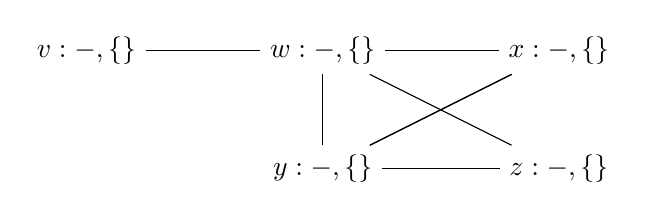
\begin{tikzpicture}[baseline=(current  bounding  box.center)]
\node (v) at (0,0)    {$v:-,\{\}$};
\node (w) at (3,0)    {$w:-,\{\}$};
\node (x) at (6,0)    {$x:-,\{\}$};
\node (y) at (3,-1.5) {$y:-,\{\}$};
\node (z) at (6,-1.5) {$z:-,\{\}$};
\draw (v) to (w);
\foreach \i in {w,x,y} 
{
  \foreach \j in {w,x,y}
  { 
    \draw (\i) to (\j);
  }
}
\draw (z) to (w);
\draw (z) to (y);
\end{tikzpicture}
\]
We select a maximally saturated node and color it $0$. In this case we
have a 5-way tie, so we arbitrarily pick $y$. The then mark color $0$
as no longer available for $w$, $x$, and $z$ because they interfere
with $y$.
\[
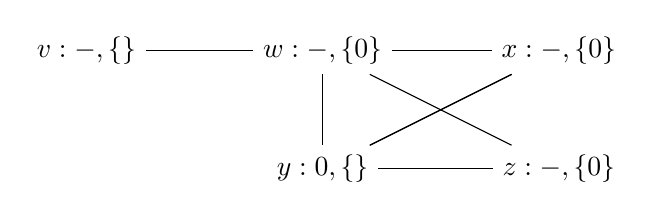
\begin{tikzpicture}[baseline=(current  bounding  box.center)]
\node (v) at (0,0)    {$v:-,\{\}$};
\node (w) at (3,0)    {$w:-,\{0\}$};
\node (x) at (6,0)    {$x:-,\{0\}$};
\node (y) at (3,-1.5) {$y:0,\{\}$};
\node (z) at (6,-1.5) {$z:-,\{0\}$};
\draw (v) to (w);
\foreach \i in {w,x,y} 
{
  \foreach \j in {w,x,y}
  { 
    \draw (\i) to (\j);
  }
}
\draw (z) to (w);
\draw (z) to (y);
\end{tikzpicture}
\]
Now we repeat the process, selecting another maximally saturated node.
This time there is a three-way tie between $w$, $x$, and $z$. We color
$w$ with $1$.
\[
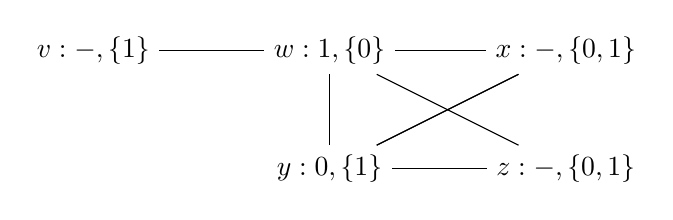
\begin{tikzpicture}[baseline=(current  bounding  box.center)]
\node (v) at (0,0)    {$v:-,\{1\}$};
\node (w) at (3,0)    {$w:1,\{0\}$};
\node (x) at (6,0)    {$x:-,\{0,1\}$};
\node (y) at (3,-1.5) {$y:0,\{1\}$};
\node (z) at (6,-1.5) {$z:-,\{0,1\}$};
\draw (v) to (w);
\foreach \i in {w,x,y} 
{
  \foreach \j in {w,x,y}
  { 
    \draw (\i) to (\j);
  }
}
\draw (z) to (w);
\draw (z) to (y);
\end{tikzpicture}
\]
The most saturated nodes are now $x$ and $z$. We color $x$ with the
next available color which is $2$.
\[
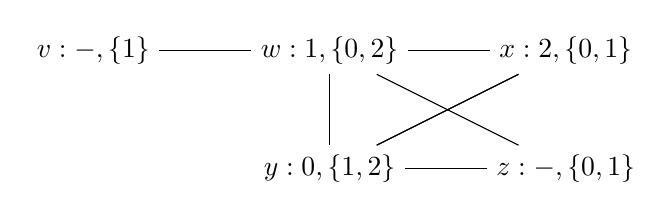
\begin{tikzpicture}[baseline=(current  bounding  box.center)]
\node (v) at (0,0)    {$v:-,\{1\}$};
\node (w) at (3,0)    {$w:1,\{0,2\}$};
\node (x) at (6,0)    {$x:2,\{0,1\}$};
\node (y) at (3,-1.5) {$y:0,\{1,2\}$};
\node (z) at (6,-1.5) {$z:-,\{0,1\}$};
\draw (v) to (w);
\foreach \i in {w,x,y} 
{
  \foreach \j in {w,x,y}
  { 
    \draw (\i) to (\j);
  }
}
\draw (z) to (w);
\draw (z) to (y);
\end{tikzpicture}
\]
We have only two nodes left to color, $v$ and $z$, but $z$ is
more highly saturated, so we color $z$ with $2$.
\[
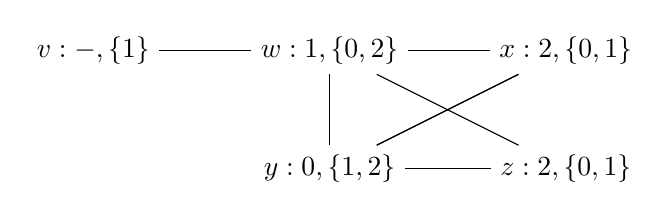
\begin{tikzpicture}[baseline=(current  bounding  box.center)]
\node (v) at (0,0)   {$v:-,\{1\}$};
\node (w) at (3,0)   {$w:1,\{0,2\}$};
\node (x) at (6,0)   {$x:2,\{0,1\}$};
\node (y) at (3,-1.5)  {$y:0,\{1,2\}$};
\node (z) at (6,-1.5)  {$z:2,\{0,1\}$};
\draw (v) to (w);
\foreach \i in {w,x,y} 
{
  \foreach \j in {w,x,y}
  { 
    \draw (\i) to (\j);
  }
}
\draw (z) to (w);
\draw (z) to (y);
\end{tikzpicture}
\]
The last iteration of the coloring algorithm assigns color $0$ to $v$.
\[
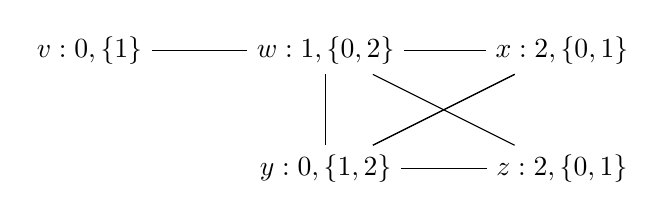
\begin{tikzpicture}[baseline=(current  bounding  box.center)]
\node (v) at (0,0)   {$v:0,\{1\}$};
\node (w) at (3,0)   {$w:1,\{0,2\}$};
\node (x) at (6,0)   {$x:2,\{0,1\}$};
\node (y) at (3,-1.5)  {$y:0,\{1,2\}$};
\node (z) at (6,-1.5)  {$z:2,\{0,1\}$};
\draw (v) to (w);
\foreach \i in {w,x,y} 
{
  \foreach \j in {w,x,y}
  { 
    \draw (\i) to (\j);
  }
}
\draw (z) to (w);
\draw (z) to (y);
\end{tikzpicture}
\]
With the coloring complete, we can finalize the assignment of
variables to registers and stack locations. Recall that if we have $k$
registers, we map the first $k$ colors to registers and the rest to
stack locations.  Suppose for the moment that we just have one extra
register to use for register allocation, just \key{rbx}. Then the
following is the mapping of colors to registers and stack allocations.
\[
  \{ 0 \mapsto \key{\%rbx}, \; 1 \mapsto \key{-8(\%rbp)}, \; 2 \mapsto \key{-16(\%rbp)}, \ldots \}
\]
Putting this together with the above coloring of the variables, we
arrive at the following assignment.
\[
  \{ v \mapsto \key{\%rbx}, \;
  w \mapsto \key{-8(\%rbp)},  \;
  x \mapsto \key{-16(\%rbp)}, \;
  y \mapsto \key{\%rbx},  \;
  z\mapsto \key{-16(\%rbp)} \}
\]
Applying this assignment to our running example
(Figure~\ref{fig:reg-eg}) yields the following program.
% why frame size of 32? -JGS
\begin{lstlisting}
(program 32
  (movq (int 1) (reg rbx))
  (movq (int 46) (stack -8))
  (movq (reg rbx) (stack -16))
  (addq (int 7) (stack -16))
  (movq (stack 16) (reg rbx))
  (addq (int 4) (reg rbx))
  (movq (stack -16) (stack -16))
  (addq (stack -8) (stack -16))
  (movq (stack -16) (reg rax))
  (subq (reg rbx) (reg rax)))
\end{lstlisting}
This program is almost an x86-64 program. The remaining step is to apply
the patch instructions pass. In this example, the trivial move of
\code{-16(\%rbp)} to itself is deleted and the addition of
\code{-8(\%rbp)} to \key{-16(\%rbp)} is fixed by going through
\code{rax}. The following shows the portion of the program that
changed.
\begin{lstlisting}
  (addq (int 4) (reg rbx))
  (movq (stack -8) (reg rax)
  (addq (reg rax) (stack -16))
\end{lstlisting}
An overview of all of the passes involved in register allocation is
shown in Figure~\ref{fig:reg-alloc-passes}.

\begin{figure}[tbp]
\[
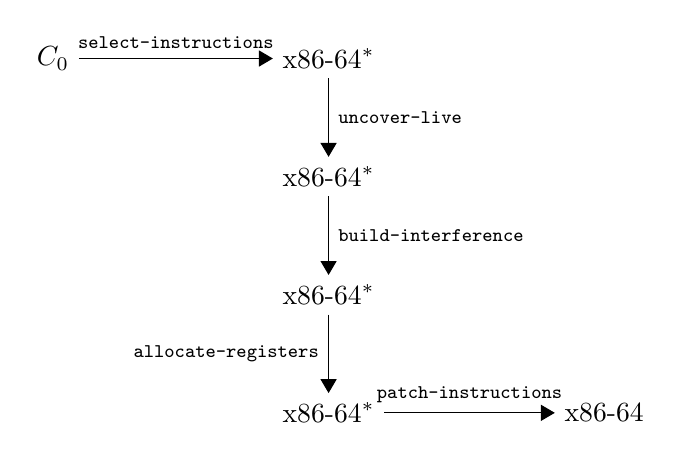
\begin{tikzpicture}[baseline=(current  bounding  box.center)]
\node (1) at (-3.5,0)     {$C_0$};
\node (2)  at (0,0)     {$\text{x86-64}^{*}$};
\node (3)  at (0,-1.5)  {$\text{x86-64}^{*}$};
\node (4)  at (0,-3)    {$\text{x86-64}^{*}$};
\node (5)  at (0,-4.5)  {$\text{x86-64}^{*}$};
\node (6)  at (3.5,-4.5)  {$\text{x86-64}$};

\path[->] (1) edge [above] node {\ttfamily\scriptsize select-instructions} (2);
\path[->] (2) edge [right] node {\ttfamily\scriptsize uncover-live}       (3);
\path[->] (3) edge [right] node {\ttfamily\scriptsize build-interference} (4);
\path[->] (4) edge [left]  node {\ttfamily\scriptsize allocate-registers} (5);
\path[->] (5) edge [above] node {\ttfamily\scriptsize patch-instructions} (6);
\end{tikzpicture}
\]
\caption{Diagram of the passes for register allocation.}
\label{fig:reg-alloc-passes}
\end{figure}

\begin{exercise}\normalfont
Implement the pass \code{allocate-registers} and test it by creating
new example programs that exercise all of the register allocation
algorithm, such as forcing variables to be spilled to the stack.

I recommend organizing our code by creating a helper function named
\code{allocate-homes} that takes an interference graph, a list of all
the variables in the program, and the list of statements. This
function should return a mapping of variables to their homes
(registers or stack locations) and the total size needed for the
stack. By creating this helper function, we will be able to reuse it
in Chapter~\ref{ch:functions} when we add support for functions.

Once you have obtained the mapping from \code{allocate-homes}, you can
use the \code{assign-homes} function from Section~\ref{sec:assign-s0}
to replace the variables with their homes.
\end{exercise}


%%%%%%%%%%%%%%%%%%%%%%%%%%%%%%%%%%%%%%%%%%%%%%%%%%%%%%%%%%%%%%%%%%%%%%%%%%%%%%%%
\chapter{Booleans, Type Checking, and Control Flow}
\label{ch:bool-types}

\section{The $R_2$ Language}

\begin{figure}[htbp]
\centering
\fbox{
\begin{minipage}{0.85\textwidth}
\[
\begin{array}{lcl}
  \Op  &::=& \ldots \mid \key{and} \mid \key{or} \mid \key{not} \mid \key{eq?} \\
  \Exp &::=& \ldots \mid \key{\#t} \mid \key{\#f} \mid
      \IF{\Exp}{\Exp}{\Exp}
\end{array}
\]
\end{minipage}
}
\caption{The $R_2$ language, an extension of $R_1$
  (Figure~\ref{fig:r1-syntax}).}
\label{fig:r2-syntax}
\end{figure}

\section{Type Checking $R_2$ Programs}

\marginpar{\scriptsize Type checking is a difficult thing to cover, I think, without having 522 as a prerequisite for this course. -- Cam}
% T ::= Integer | Boolean

It is common practice to specify a type system by writing rules for
each kind of AST node. For example, the rule for \key{if} is:
\begin{quote}
  For any expressions $e_1, e_2, e_3$ and any type $T$, if $e_1$ has
  type \key{bool}, $e_2$ has type $T$, and $e_3$ has type $T$, then
  $\IF{e_1}{e_2}{e_3}$ has type $T$.
\end{quote}
It is also common practice to write rules using a horizontal line,
with the conditions written above the line and the conclusion written
below the line.
\begin{equation*}
  \inference{e_1 \text{ has type } \key{bool} & 
        e_2 \text{ has type } T & e_3 \text{ has type } T}
  {\IF{e_1}{e_2}{e_3} \text{ has type } T}
\end{equation*}
Because the phrase ``has type'' is repeated so often in these type
checking rules, it is abbreviated to just a colon. So the above rule
is abbreviated to the following.
\begin{equation*}
  \inference{e_1 : \key{bool} & e_2 : T & e_3 : T}
            {\IF{e_1}{e_2}{e_3} : T}
\end{equation*}

The $\LET{x}{e_1}{e_2}$ construct poses an interesting challenge. The
variable $x$ is assigned the value of $e_1$ and then $x$ can be used
inside $e_2$. When we get to an occurrence of $x$ inside $e_2$, how do
we know what type the variable should be?  The answer is that we need
a way to map from variable names to types.  Such a mapping is called a
\emph{type environment} (aka. \emph{symbol table}). The capital Greek
letter gamma, written $\Gamma$, is used for referring to type
environments environments. The notation $\Gamma, x : T$ stands for
making a copy of the environment $\Gamma$ and then associating $T$
with the variable $x$ in the new environment.  We write $\Gamma(x)$ to
lookup the associated type for $x$.  The type checking rules for
\key{let} and variables are as follows.
\begin{equation*}
  \inference{e_1 : T_1 \text{ in } \Gamma &
             e_2 : T_2 \text{ in } \Gamma,x:T_1}
            {\LET{x}{e_1}{e_2} : T_2 \text{ in } \Gamma} 
  \qquad
  \inference{\Gamma(x) = T}
            {x : T \text{ in } \Gamma}
\end{equation*}
Type checking has roots in logic, and logicians have a tradition of
writing the environment on the left-hand side and separating it from
the expression with a turn-stile ($\vdash$).  The turn-stile does not
have any intrinsic meaning per se.  It is punctuation that separates
the environment $\Gamma$ from the expression $e$.  So the above typing
rules are written as follows.
\begin{equation*}
  \inference{\Gamma \vdash e_1 : T_1 &
             \Gamma,x:T_1 \vdash e_2 : T_2}
            {\Gamma \vdash \LET{x}{e_1}{e_2} : T_2} 
   \qquad
  \inference{\Gamma(x) = T}
            {\Gamma \vdash x : T}
\end{equation*}
Overall, the statement $\Gamma \vdash e : T$ is an example of what is
called a \emph{judgment}.  In particular, this judgment says, ``In
environment $\Gamma$, expression $e$ has type $T$.''
Figure~\ref{fig:S1-type-system} shows the type checking rules for
$R_2$.

\begin{figure}
\begin{gather*}
  \inference{\Gamma(x) = T}
            {\Gamma \vdash x : T}
   \qquad
  \inference{\Gamma \vdash e_1 : T_1 &
             \Gamma,x:T_1 \vdash e_2 : T_2}
            {\Gamma \vdash \LET{x}{e_1}{e_2} : T_2} 
  \\[2ex]
  \inference{}{\Gamma \vdash n : \key{Integer}}
  \quad
  \inference{\Gamma \vdash e_i : T_i \ ^{\forall i \in 1\ldots n} & \Delta(\Op,T_1,\ldots,T_n) = T}
            {\Gamma \vdash (\Op \; e_1 \ldots e_n) : T}
  \\[2ex]
  \inference{}{\Gamma \vdash \key{\#t} : \key{Boolean}}
  \quad
  \inference{}{\Gamma \vdash \key{\#f} : \key{Boolean}}
  \quad
  \inference{\Gamma \vdash e_1 : \key{bool} \\
             \Gamma \vdash e_2 : T &
             \Gamma \vdash e_3 : T}
  {\Gamma \vdash \IF{e_1}{e_2}{e_3} : T}
\end{gather*}
\caption{Type System for $R_2$.}
\label{fig:S1-type-system}
\end{figure}


\begin{figure}

\begin{align*}
\Delta(\key{+},\key{Integer},\key{Integer}) &= \key{Integer} \\
\Delta(\key{-},\key{Integer},\key{Integer}) &= \key{Integer} \\
\Delta(\key{-},\key{Integer}) &= \key{Integer} \\
\Delta(\key{*},\key{Integer},\key{Integer}) &= \key{Integer} \\
\Delta(\key{read}) &= \key{Integer} \\
\Delta(\key{and},\key{Boolean},\key{Boolean}) &= \key{Boolean} \\
\Delta(\key{or},\key{Boolean},\key{Boolean}) &= \key{Boolean} \\
\Delta(\key{not},\key{Boolean}) &= \key{Boolean} \\
\Delta(\key{eq?},\key{Integer},\key{Integer}) &= \key{Boolean} \\
\Delta(\key{eq?},\key{Boolean},\key{Boolean}) &= \key{Boolean} 
\end{align*}

\caption{Types for the primitives operators.}
\end{figure}


\section{The $C_1$ Language}

\begin{figure}[htbp]
\[
\begin{array}{lcl}
\Arg &::=& \ldots \mid \key{\#t} \mid \key{\#f} \\
\Stmt &::=& \ldots \mid \IF{\Exp}{\Stmt^{*}}{\Stmt^{*}} 
\end{array}
\]
\caption{The $C_1$ intermediate language, an extension of $C_0$
  (Figure~\ref{fig:c0-syntax}).}
\label{fig:c1-syntax}
\end{figure}

\section{Flatten Expressions}

\section{Select Instructions}

\section{Register Allocation}

\section{Patch Instructions}


%%%%%%%%%%%%%%%%%%%%%%%%%%%%%%%%%%%%%%%%%%%%%%%%%%%%%%%%%%%%%%%%%%%%%%%%%%%%%%%%
\chapter{Tuples and Heap Allocation}
\label{ch:tuples}

%%%%%%%%%%%%%%%%%%%%%%%%%%%%%%%%%%%%%%%%%%%%%%%%%%%%%%%%%%%%%%%%%%%%%%%%%%%%%%%%
\chapter{Garbage Collection}
\label{ch:gc}


%%%%%%%%%%%%%%%%%%%%%%%%%%%%%%%%%%%%%%%%%%%%%%%%%%%%%%%%%%%%%%%%%%%%%%%%%%%%%%%%
\chapter{Functions}
\label{ch:functions}


%%%%%%%%%%%%%%%%%%%%%%%%%%%%%%%%%%%%%%%%%%%%%%%%%%%%%%%%%%%%%%%%%%%%%%%%%%%%%%%%
\chapter{Lexically Scoped Functions}
\label{ch:lambdas}


%%%%%%%%%%%%%%%%%%%%%%%%%%%%%%%%%%%%%%%%%%%%%%%%%%%%%%%%%%%%%%%%%%%%%%%%%%%%%%%%
\chapter{Mutable Data}
\label{ch:mutable-data}

%%%%%%%%%%%%%%%%%%%%%%%%%%%%%%%%%%%%%%%%%%%%%%%%%%%%%%%%%%%%%%%%%%%%%%%%%%%%%%%%
\chapter{The Dynamic Type}
\label{ch:type-dynamic}


%%%%%%%%%%%%%%%%%%%%%%%%%%%%%%%%%%%%%%%%%%%%%%%%%%%%%%%%%%%%%%%%%%%%%%%%%%%%%%%%
\chapter{Parametric Polymorphism}
\label{ch:parametric-polymorphism}

%%%%%%%%%%%%%%%%%%%%%%%%%%%%%%%%%%%%%%%%%%%%%%%%%%%%%%%%%%%%%%%%%%%%%%%%%%%%%%%%
\chapter{High-level Optimization}
\label{ch:high-level-optimization}

%%%%%%%%%%%%%%%%%%%%%%%%%%%%%%%%%%%%%%%%%%%%%%%%%%%%%%%%%%%%%%%%%%%%%%%%%%%%%%%%
\chapter{Appendix}

\section{Interpreters}
\label{appendix:interp}

We provide several interpreters in the \key{interp.rkt} file.  The
\key{interp-scheme} function takes an AST in one of the Racket-like
languages considered in this book ($R_1, R_2, \ldots$) and interprets
the program, returning the result value.  The \key{interp-C} function
interprets an AST for a program in one of the C-like languages ($C_0,
C_1, \ldots$), and the \key{interp-x86} function interprets an AST for
an x86-64 program.

\section{Utility Functions}
\label{appendix:utilities}

The utility function described in this section can be found in the
\key{utilities.rkt} file.

The \key{assert} function displays the error message \key{msg} if the
Boolean \key{bool} is false.
\begin{lstlisting}
(define (assert msg bool) ...)
\end{lstlisting}

The \key{lookup} function ...

The \key{map2} function ...

The \code{make-graph}, \code{add-edge}, and \code{adjacent}
functions...

The \key{interp-tests} function takes a compiler name (a string) a
description of the passes a test family name (a string), and a list of
test numbers, and runs the compiler passes and the interpreters to
check whether the passes correct. The description of the passes is a
list with one entry per pass.  An entry is a list with three things: a
string giving the name of the pass, the function that implements the
pass (a translator from AST to AST), and a function that implements
the interpreter (a function from AST to result value).  The
interpreters from Appendix~\ref{appendix:interp} make a good choice.
The \key{interp-tests} function assumes that the subdirectory
\key{tests} has a bunch of Scheme programs whose names all start with
the family name, followed by an underscore and then the test number,
ending in \key{.scm}. Also, for each Scheme program there is a file
with the same number except that it ends with \key{.in} that provides
the input for the Scheme program.
\begin{lstlisting}
(define (interp-tests name passes test-family test-nums) ...
\end{lstlisting}

The compiler-tests function takes a compiler name (a string) a
description of the passes (see the comment for \key{interp-tests}) a
test family name (a string), and a list of test numbers (see the
comment for interp-tests), and runs the compiler to generate x86-64 (a
\key{.s} file) and then runs gcc to generate machine code.  It runs
the machine code and checks that the output is 42.
\begin{lstlisting}
(define (compiler-tests name passes test-family test-nums) ...)
\end{lstlisting}

The compile-file function takes a description of the compiler passes
(see the comment for \key{interp-tests}) and returns a function that,
given a program file name (a string ending in \key{.scm}), applies all
of the passes and writes the output to a file whose name is the same
as the proram file name but with \key{.scm} replaced with \key{.s}.
\begin{lstlisting}
(define (compile-file passes)
  (lambda (prog-file-name) ...))
\end{lstlisting}

\bibliographystyle{plainnat}
\bibliography{all}

\end{document}

%%  LocalWords:  Dybvig Waddell Abdulaziz Ghuloum Dipanwita
%%  LocalWords:  Sarkar lcl Matz aa representable
